%%%%%%%%%%%%%%%%%%%%%%%%%%%%%%%%%
% 6CCS3PRJ Final Year Individual Project Report
% luke.day@kcl.ac.uk
%%%%%%%%%%%%%%%%%%%%%%%%%%%%%%%%%
\documentclass[12pt]{informatics-report}
\usepackage{color}
\usepackage[square,sort,comma,numbers]{natbib}
\usepackage[utf8]{inputenc}
\usepackage{listings}
\usepackage{indentfirst}
\usepackage{longtable}
\usepackage{titlesec}
\definecolor{lightgray}{rgb}{.97,.97,.97}
\definecolor{darkgray}{rgb}{.4,.4,.4}
\definecolor{purple}{rgb}{0.65, 0.12, 0.82}
\usepackage{float}
%\floatstyle{boxed}
\restylefloat{figure}

\lstdefinelanguage{JavaScript}{
  keywords={typeof, new, true, false, catch, function, return, null, catch, switch, var, if, in, while, do, else, case, break},
  keywordstyle=\color{blue}\bfseries,
  ndkeywords={class, export, boolean, throw, implements, import, this},
  ndkeywordstyle=\color{darkgray}\bfseries,
  identifierstyle=\color{black},
  sensitive=false,
  comment=[l]{//},
  morecomment=[s]{/*}{*/},
  commentstyle=\color{purple}\ttfamily,
  stringstyle=\color{red}\ttfamily,
  morestring=[b]',
  morestring=[b]"
}

\lstset{
   language=JavaScript,
   backgroundcolor=\color{lightgray},
   extendedchars=true,
   basicstyle=\footnotesize\ttfamily,
   showstringspaces=false,
   showspaces=false,
   numbers=left,
   numberstyle=\footnotesize,
   numbersep=9pt,
   tabsize=2,
   breaklines=true,
   showtabs=false,
   captionpos=b
}


 %References
%%%%%%%%%%%%%%%%%%%%%%%%%%%%%%%%%
% Front Matter - project title, name, supervisor name and date
%%%%%%%%%%%%%%%%%%%%%%%%%%%%%%%%%
\title{6CCS3PRJ\\\vspace{0.2cm}Dining Cryptographers Network Simulation Tool}
\author{Federico Capaldo}
\studentID{1444686}
\supervisor{Professor Luca Viganó}

\date{\today}

\abstractFile{FrontMatter/abstract.tex}
\ackFile{FrontMatter/acknowledgements.tex} %Remove line if you do not want acknowledgements


\titleformat{\subparagraph}
    {\normalfont\normalsize\bfseries}{\thesubparagraph}{1em}{}
\titlespacing*{\subparagraph}{\parindent}{3.25ex plus 1ex minus .2ex}{.75ex plus .1ex}

\begin{document}
{%
\setlength{\fboxsep}{0pt}%
\setlength{\fboxrule}{1pt}%
}%

\setcounter{secnumdepth}{5}

\createFrontMatter
\onehalfspacing
\tableofcontents
\doublespacing



%%%%%%%%%%%%%%%%%%%%%%%%%%%%%%%%%
% Report Content
%%%%%%%%%%%%%%%%%%%%%%%%%%%%%%%%%
% You can write each chapter directly here or in a separate .tex file and use the include command.

\chapter{Introduction}


To protect people's privacy and freedom of speech, different protocols have been developed in an attempt to provide untraceable communication. Untraceability can be understood as the inability to link an action to the principal who performed it. Among the protocols that fulfill such security goal, the Dining Cryptographers Network (DC-Net) is the strongest one to provide untraceability of the sender and receiver. 

What makes DC-Net particularly interesting is its property of unconditional security: the protocol is invulnerable to any kind crypto-analytic attack, no matter the amount of computational power of an adversary. This property holds in theory very well. However, the protocol is generally deemed impractical. Thus, there are very few attempts to simulate it.

Current simulations of DC-Net do not follow the distributed architecture of the protocol, and they are not usable in the real world. Some of them are inaccessible to the user due to cumbersome setup and have a poor user interface.

This project attempts to simulate the protocol faithfully to the theory. In particular, it tries to preserve sender untraceability at all times. By doing so, I aim to demonstrate some of the difficulties of implementing a perfectly secure protocol.

\section{Motivation}
The drive to create a simulation for this protocol is three-fold: 

\begin{enumerate}
\item Despite being the most secure protocol in terms of untraceability, DC-Net presents limitations for real-world implementations that can be addressed;

\item There is a scarce number of projects aimed at simulating the protocol for academics interested in the topic;

\item This project allows me to further explore my interest in Information Security, an area of Computer Science that fascinates me due to the socio-political implications around personal privacy. Moreover, the core idea of a DC-Net is a simple the XOR logic operation (explained in the main body). There is a certain beauty that arises from the fact that applying a simple concept gives life to a protocol that guarantees unconditional security.
\end{enumerate}


\section{Project Scope}
The project focuses on a simulation of the Dining Cryptographer protocol at a practical level. I concentrate on the protocol's ability to guarantee sender anonymity. 

In addition to the simulation tool, part of the scope of this project is to also analyse the challenges encountered first-hand during the implementation. 

I do not treat the issue of detecting collusion of participants.  Moreover, although I provide a solution to exchange secret keys securely, I do not address this issue at a protocol level.


\section{Solution Objectives}
The project undertaken has the purpose of building a simulation tool to demonstrate the functioning of the Dining Cryptographer protocol to those who would like to acquire a pragmatic understanding of it.

The solution consists of a web application, designed to ease its access and usage, by removing possible installation steps that a native application may have required. Moreover, it employs a client-server architecture. The server entity facilitates the implementation of a real distributed system, and helps the exchange of messages between participants.

Although this is a real-time application so multiple clients can communicate instantaneously, delays are intentionally introduced in the execution of the protocol to help the users understand how the protocol works step-by-step. 

In line with this educational objective of the simulation tool, I design a GUI so that the simulator is user-friendly. In this way, the user should find the application instructive in the process of deepening their knowledge of a DC-Net.


\section{Target Audience}
The intended audience of this project is academics and Information Security students interested in the workings of the DC-Net protocol. Overall, I assume the target audience to be highly computer literate at university level.


\section{Personal Contributions}
With the delivery of this project, my contributions to the academic discussion on the DC-Net topic are listed below. \newline

Firstly, the simulation tool implemented is unique in its kind as, to my knowledge, there is no other user-friendly interface application that simulates this theoretical protocol. Consequently, I do not use a command-line tool as this does not offer an intuitive UI.  Moreover, what renders it unique is that I actually deploy the tool as a distributed system rather than simulating the network on a single machine. The simulation is available online at \url{https://dc-net.herokuapp.com}. \newline

Secondly, the experience of building this simulator from scratch has been an authentic journey of self-learning. Thanks to this, I have observed first-hand some of the complex challenges of translating a theoretical security protocol into a deployed piece of work.
Put together, my analysis on the work performed represent a complementary contribution to the academic debate on the DC-Net protocol, the latter focusing entirely on theoretical considerations. \newline


Lastly, given the lack of examples on how to implement a DC-Net, I put forward specific solutions that aim to further bridge the gap between theory and real-world usage of the protocol. Specifically, I propose to interpret round messages with Extended ASCII encoding standard, which enables the transmission of human readable messages. I also introduce the concept of length-calculation round as an intermediate step to voting and communication rounds to preserve untraceability when a message is communicated across multiple rounds. Finally, I try to guarantee a degree of fairness in the network usage by preventing the same user from sending back-to-back.


\section{Report Structure}

The report consists of 8 chapters and its content is presented as it follows:

In chapter 1, the current chapter, I outline the motivation, scope and objectives of the simulation tool.

In chapter 2, I review the differences between anonymity and untraceability, which sets the scene for an in-depth presentation of the DC-Net protocol. I, then, explain the limitations and possible extensions of the basic protocol and review the current state of art of the DC-Net implementations.

In chapter 3, I present the basic and advanced requirements of the application. Following, I present how each requirement is fulfilled in the implementation. 

In chapter 4, I motivate the design choices taken and present the design of the implemented simulation by employing UML diagram notations.

In chapter 5, I delves into the actual implementation. I describe the technologies used, and provide code snippets of the main functionalities. I then outline the challenges faced throughout development and conclude with the mapping of the theoretical concepts to the corresponding features implemented.

In chapter 6, I briefly state how the piece of software implemented does not present ethical issues.

In chapter 7, I evaluate the work undertaken meets the project's requirements, I compared the work against available simulation tools and address the known limitations. I then present my analysis of the difficulties of preserving untraceability when trying to implement a Dining Cryptographer Network.

Lastly, in chapter 8, I summarise the overall project and draw the conclusion over the accomplished work and discusses possible future works.
\chapter{Background Research and Literature Review}

In Information Security, anonymity can be a difficult notion to conceptualize. This chapter begins by introducing two different aspects of anonymity so as to place this study in context. Next, it follows an in depth description of the Dining Cryptographers protocol, the main focus of the thesis, starting from a theoretical standpoint and ending with practical considerations for the suggested implementation. Lastly, the chapter will outline the current state of art of DC-Net implementations.

\section{What is Anonymity}
Generally speaking, the definition of anonymity is presented as a "lack of outstanding, individual, or unusual features." \cite{Anonymity}. In Information Security, anonymity is a security goal a system may want to achieve. Attaining such security property means that it is infeasible to hold a principal accountable for an anonymous action. In other words, anonymity prevents any principal from identifying another principal performing an action within an anonymous network \cite{Malkhi}.

An anonymity network composed of a finite set of participants is called anonymity set.

\subsection{Anonymity Set} \label{sec:anonymityset}
When considering an anonymity set, anonymity is precisely defined in relation to others: for a principal to be anonymous in doing an action, other subjects An anonymity network composed of a finite set of participants is called anonymity set \cite{Pfitzmann}.

It follows that the number of agents inside the anonymity set determines the level of anonymity that can be achieved. Therefore, anonymity is an incremental concept: the more the participants inside an anonymous network, the higher the degree of anonymity. The minimum number of principals to guarantee this property is two,as a network with one agent exhibits no anonymity whatsoever (See Figure \ref{fig:anonymity}) \cite{Franck}.

\begin{figure}[h]
    \centering
    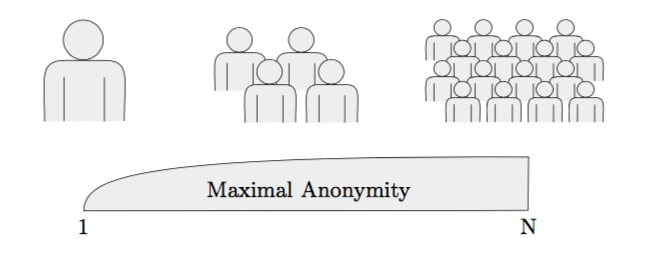
\includegraphics[width=0.50\textwidth]{Images/anonymityLevel.png}
    \caption{Level of anonymity in a set \cite{Franck}}
    \label{fig:anonymity}
\end{figure}

The features of anonymity presented above fit well with the definition of 'hiding one's identity'. 
In information security, however, considering the types of anonymity set adds another dimension to the concept. There are two types of anonymity set: sender anonymity set and recipient anonymity set. The former refers to multiple participants inside the set of senders and one, or possibly more, agents in the recipients set (figure \ref{fig:senderAnonSet}). The latter, instead, refers to the opposite scenario having many recipients in one set and one, or possibly more, senders in the other (figure \ref{fig:receipientAnonSet}).


\begin{figure}[h]
\centering
\begin{minipage}{.5\textwidth}
    \centering
    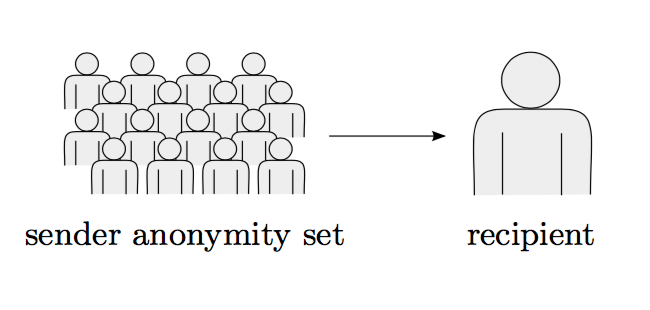
\includegraphics[width=0.50\textwidth]{Images/ReceiverAnonymSet.png}
    \caption{Sender anonymity set \cite{Franck}}
    \label{fig:senderAnonSet}
\end{minipage}%
\begin{minipage}{.5\textwidth}
    \centering
    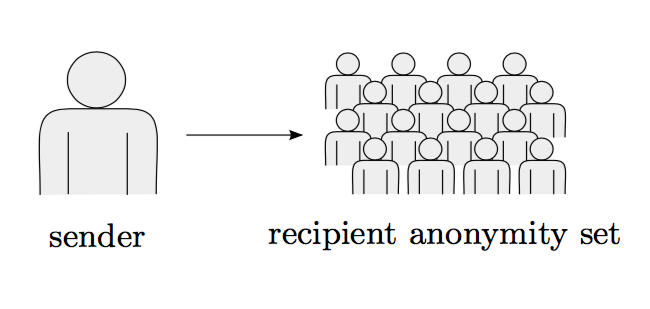
\includegraphics[width=0.50\textwidth]{Images/senderAnonymSet.png}
    \caption{Recipient anonymity set \cite{Franck}}
    \label{fig:receipientAnonSet}
\end{minipage}
\end{figure}



\begin{figure}[h]
    \centering
    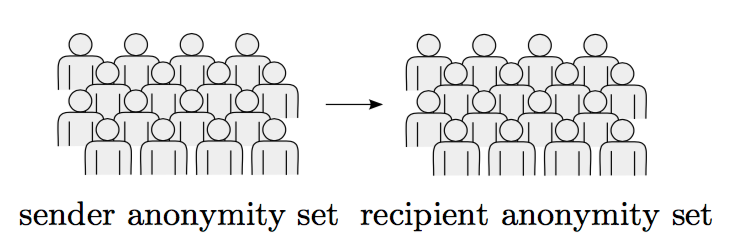
\includegraphics[width=0.50\textwidth]{Images/ManyToManyAnonymSet.png}
    \caption{Anonymity sets with multiple senders and recipients \cite{Franck}}
    \label{fig:anonymityLevel}
\end{figure}

Senders and recipients may overlap in the same set as shown in figure \ref{fig:overlappingAnonSet}.

\begin{figure}[h]
    \centering
    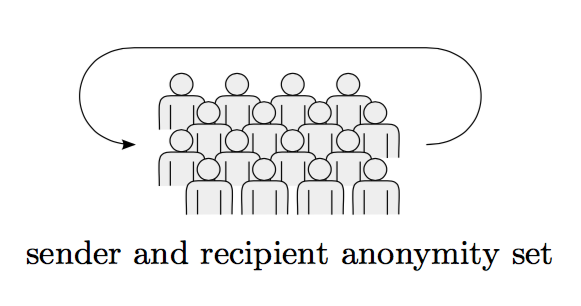
\includegraphics[width=0.50\textwidth]{Images/overlappingAnonymSet.png}
    \caption{Overlapping senders and receivers in anonymity set \cite{Franck}}
    \label{fig:overlappingAnonSet}
\end{figure}


\subsection{Identity Anonymity versus Sender/Recipient Anonymity}
When considering what anonymity means in the two types of anonymity set, the notion shifts from a participant's identity being hidden to being untraceable, i.e. an action cannot be traced back to a specific principal within the set. In fact, all senders identities and/or recipients identities can be known. However, if a principal would like to perform an action - like sending a message - all other participants also perform the same action - in this case act as senders by dispatching a dummy messages (noise) - so that it is not distinguishable which of all the messages is the real message and, as a consequence, who is the real sender.

As a result of this analysis, it follows that the classic notion of anonymity refers to hiding one's identity. However, a different concept is sender/recipient anonymity, which instead equates to the concept of untraceability. Specifically, untraceability has as its main feature the inability of determine which principal of the network, with  knowable identities, is the actual sender or recipient of a message. \newline 


In this frame of reference, the Dining Cryptographer protocol is a protocol that offers strong sender and recipient untraceability \cite{Chaum}, which is the central subject of this thesis. Therefore, at least from a theoretical standpoint, in a Dining Cryptographers Network senders and recipients are completely untraceable. 

The use of the term anonymity from now on in this document refers solely to sender/recipient anonymity, i.e. untraceability, unless explicitly stated otherwise.

\section{The Dining Cryptographers}
David Chaum first theorised this concept in "The Dining Cryptographers Problem" publication in the Journal of Cryptology in January 1988 (Volume 1, Issue 1, pp 65-75). Chaum here describes a protocol that employs one-time-use keys in order to offer unconditional sender and receiver untraceability within a network (a DC-Net) \cite{Chaum}. 

To simplify the understanding of the underlying techniques of the protocol to the reader, Chaum's analogy is presented first, followed by a more formal exposition.

\subsection{The protocol Analogy - The Dinner}
Three cryptographers decide to dine at a restaurant. At the end of the meal, the waiter informs the table that the bill has already been paid anonymously. The arrangement might have been made by one of the three dining cryptographers or by their employer, the National Security Agency (the NSA). The diners respect each other's privacy to pay anonymously, but they are interested to know if the payer is at the table or if indeed it was their employer. In order to determine the answer, they execute the following three phases \cite{Chaum}:
\begin{enumerate} \label{sec:protocolStages}
    \item Every cryptographer has one neighbour sitting on his left and one of his right. Each cryptographer tosses an unbiased coin behind a menu between him and his right neighbour so that the third participant cannot see the outcome (Figure \ref{fig:dcstage1}). At this point, each cryptographer can see the result of two coin flips, the one he flipped with his right neighbour and the one that his left neighbour flipped with him (Figure \ref{fig:dcstage2}). 
    \item Subsequently, each cryptographer states out loud whether the two coins have the same value (two heads or two tails) or otherwise (Figure \ref{fig:dcstage3}). If the cryptographer paid for the dinner, he lies about the result of the coins and says the exact contrary of what he sees.
    \item Finally, all the results of the three cryptographers are combined in order to find the truth about who paid. An even number of "Different" means that the NSA paid for the dinner, and odd number of "Different" means that one of the cryptographers at the table paid for the dinner.
\end{enumerate}

\begin{figure}[h!]
    \centering
    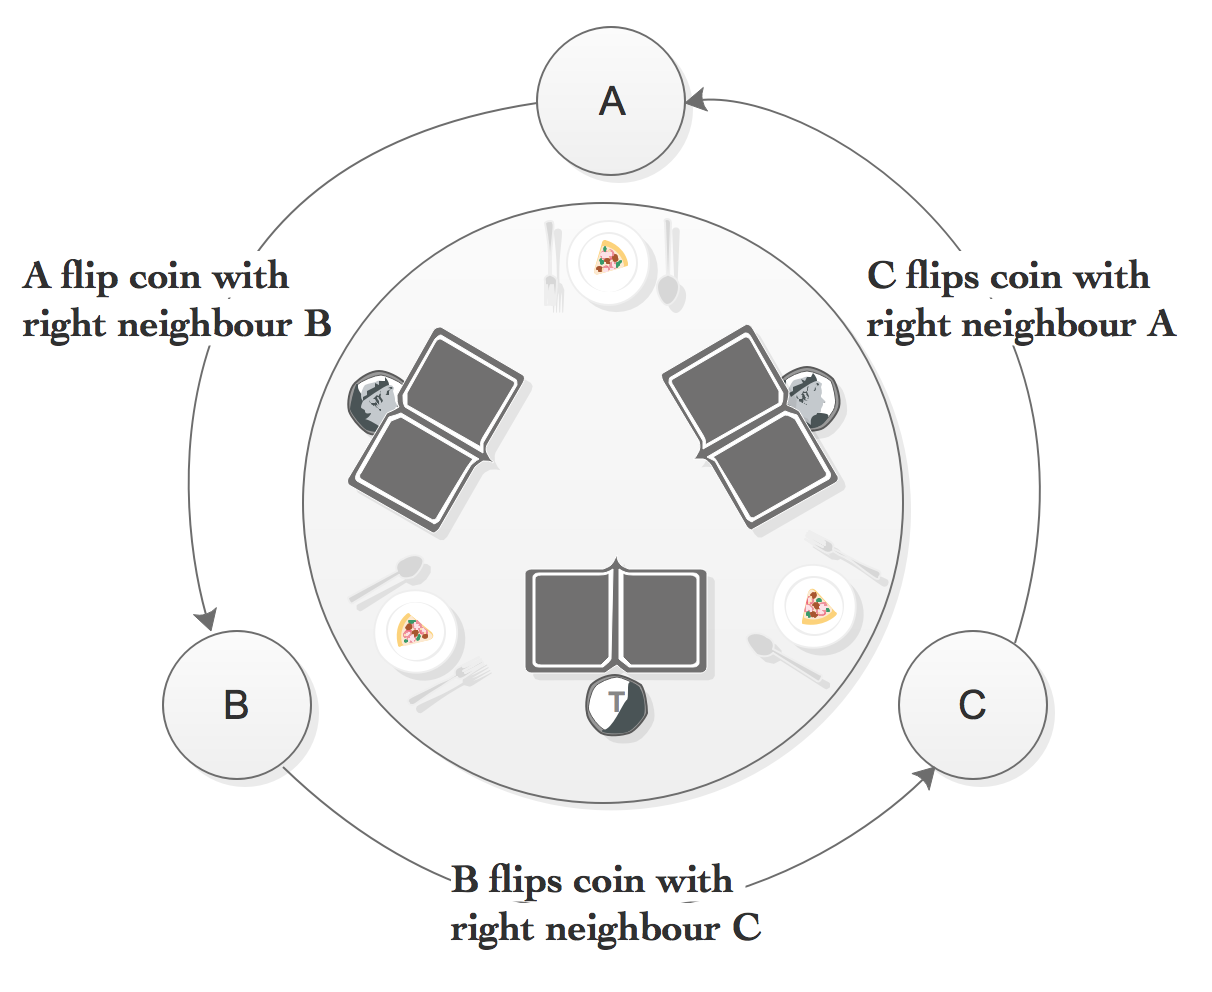
\includegraphics[width=0.50\textwidth]{Images/DCstep1.png}
    \caption{Diners flip coins}
    \label{fig:dcstage1}
\end{figure}

\begin{figure}[h!]
    \centering
    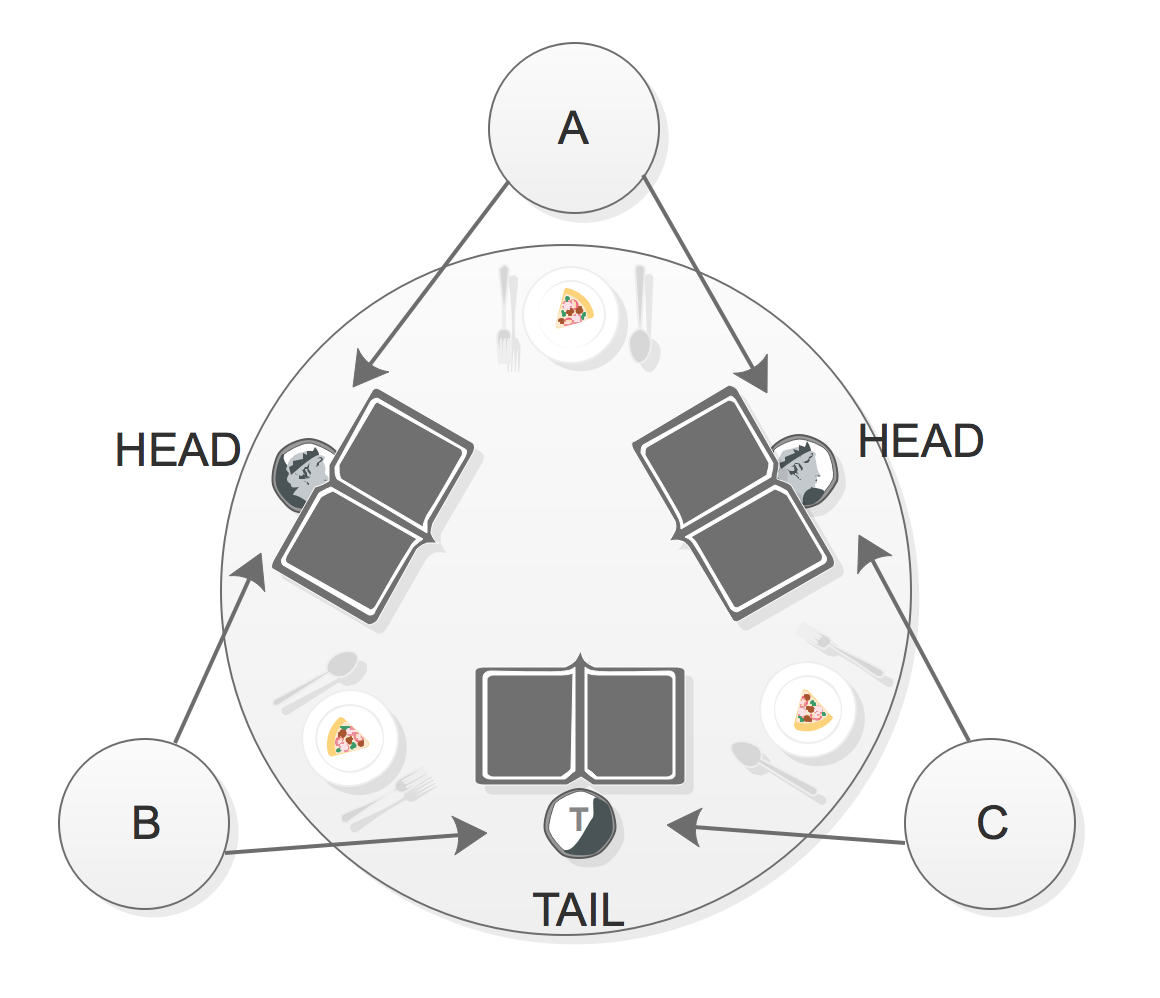
\includegraphics[width=0.50\textwidth]{Images/DCstep2.png}
    \caption{What each cryptographer can see}
    \label{fig:dcstage2}
\end{figure}

\begin{figure}[h!]
    \centering
    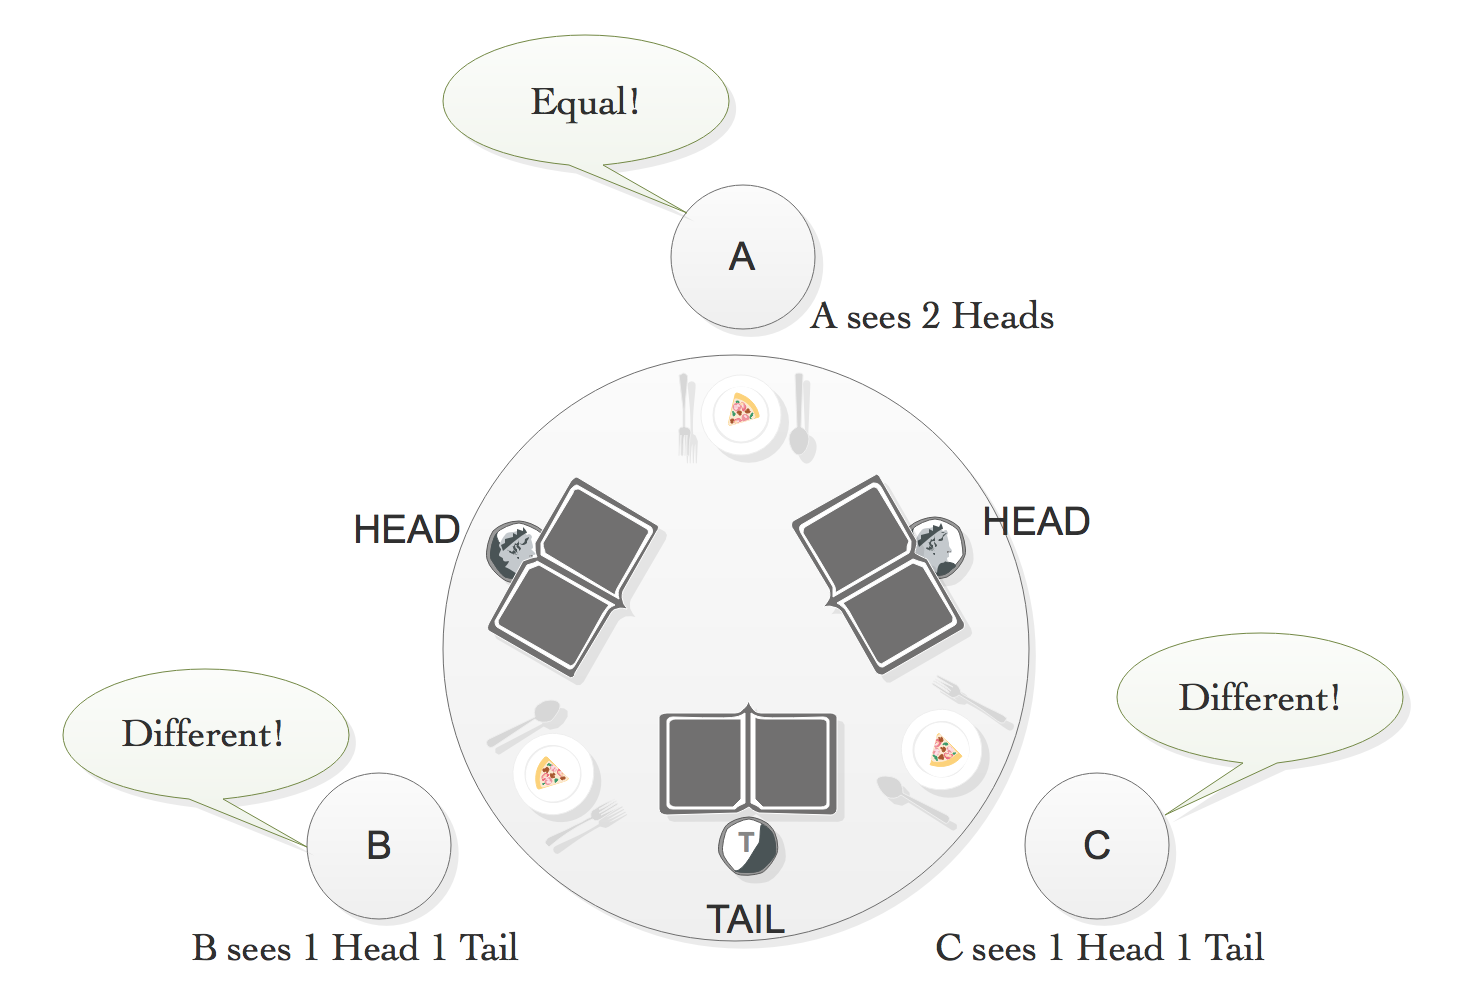
\includegraphics[width=0.70\textwidth]{Images/DCstep3NoPayers.png}
    \caption{Cryptographers broadcast responses. Even number of "Different" implies that no one is the payer.}
    \label{fig:dcstage3}
\end{figure}

To sum up, if one of the three cryptographers at the table paid for the meal, neither of the two non-paying cryptographers would gain any additional information about who, between the two other participants other than himself, might be the payer. This is because each participant does not know the outcome of the third coin flip between the other two participants.  Such is the explanation of how sender anonymity is guaranteed in the Dining Cryptographers protocol. 

Importantly, Chaum also proves how sender anonymity within this protocol is unconditionally secure in theory \cite{Chaum}. This property of the protocol makes it fascinating as it means that untraceability holds in all possible scenarios within the network.  We turn now to present how this is the case. 


\subsection{Proving Unconditional Security}
Unconditional security is a term coined by Whitfield Diffie and it entails that, no matter the amount of computational power that an attacker may have, any kind of crypto-analytic attack on this protocol is ineffective, provided that the protocol has been carried out accurately \cite{Diffie1}.

In order to understand why the Dining Cryptographer problem provides such property, all the possible scenarios need to be explored:
\begin{enumerate}
    \item If the NSA paid, there is no issue in preserving the anonymity of any of the cryptographers;
    \item The interesting cases are those whereby one of the three cryptographers is the payer. 
    
    Let us assume that a non-paying participant, called A, wishes to find out who paid the dinner. There are two cases: \begin{enumerate}
        \item subject A sees two equal coins (e.g. 2 heads). Then, if the third hidden coin is the same as what A sees, the cryptographer that said 'Different' is the payer (Figure \ref{fig:AsameCaseSame}); if the third hidden coin is different from what A sees, then the cryptographer who said 'Same' is the payer (Figure \ref{fig:AsameCaseDifferent}) \cite{Chaum};
        \begin{figure}[h!]
            \centering
            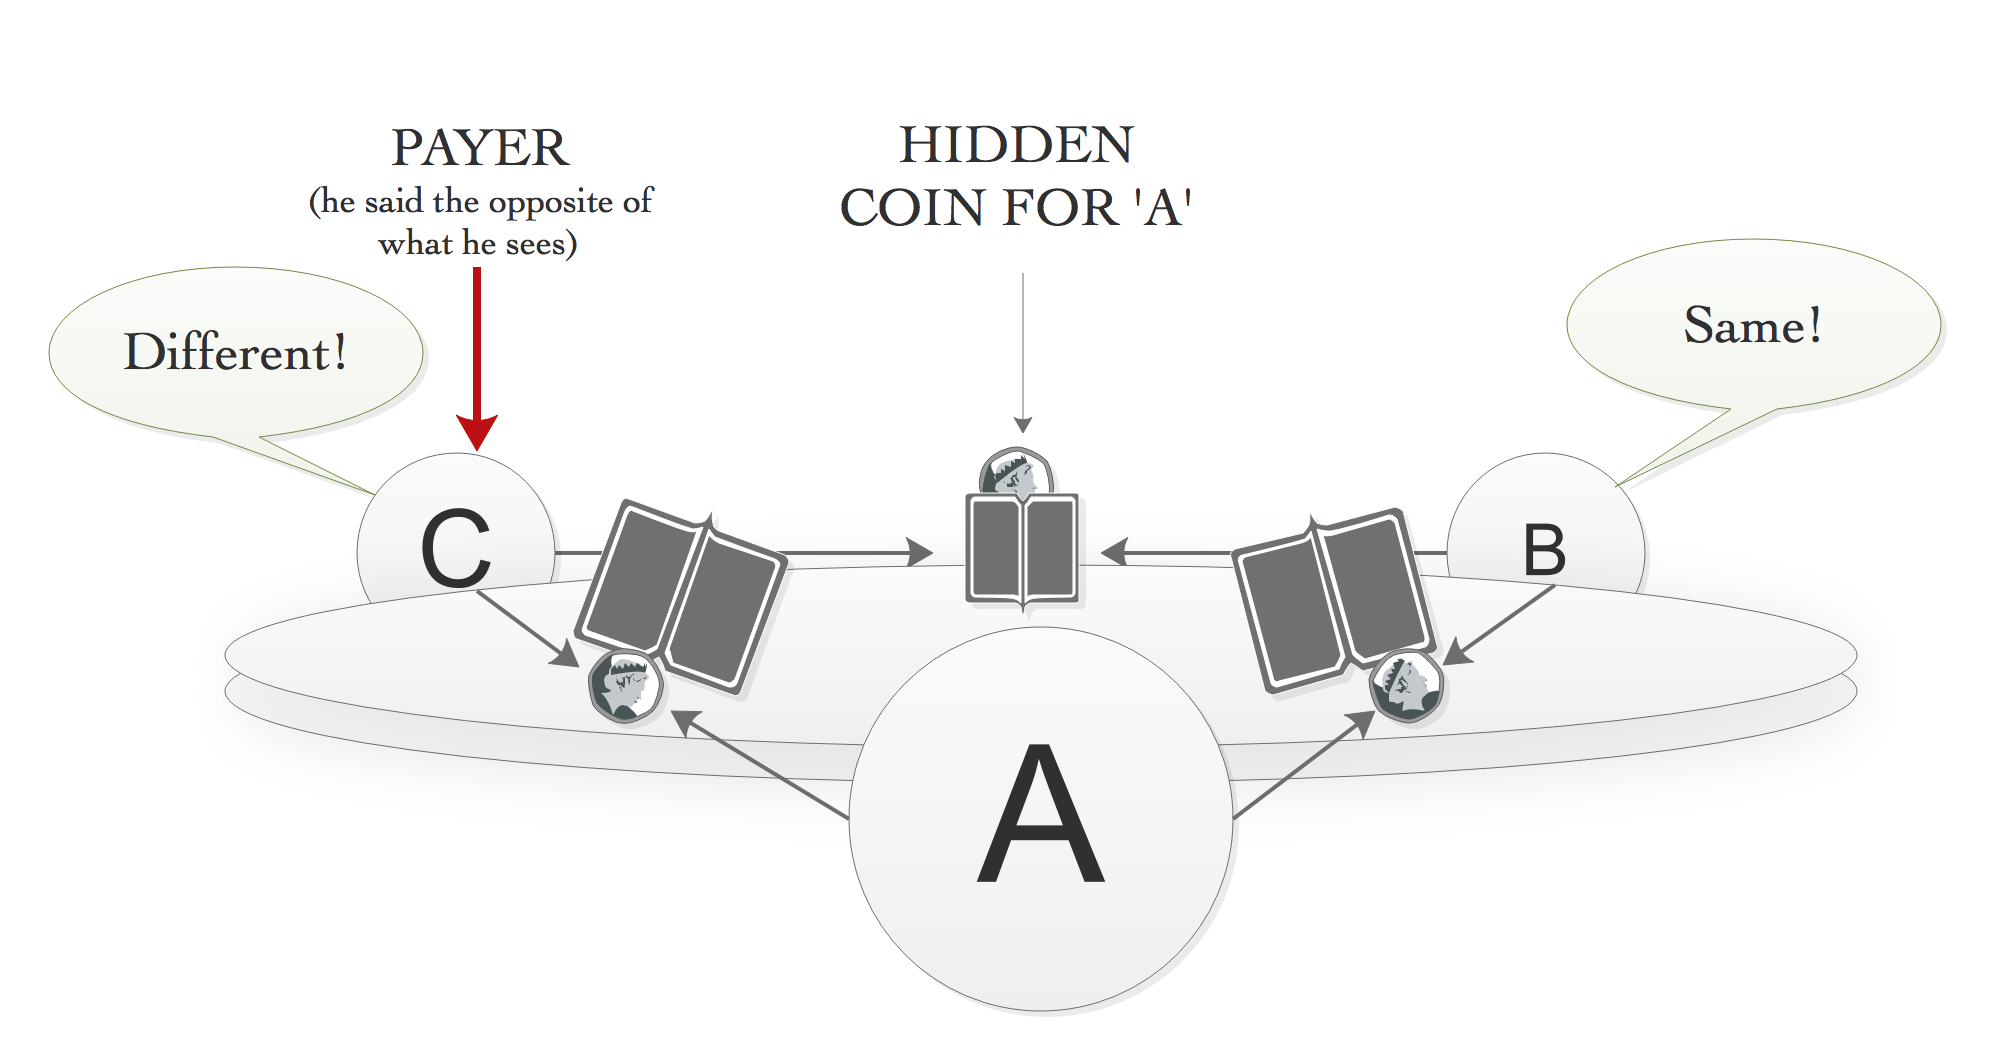
\includegraphics[width=0.80\textwidth]{Images/AsameCase1.png}
            \caption{Hidden Coin same as what A sees. C is the Payer.}
            \label{fig:AsameCaseSame}
        \end{figure}
        \begin{figure}[h!]
            \centering
            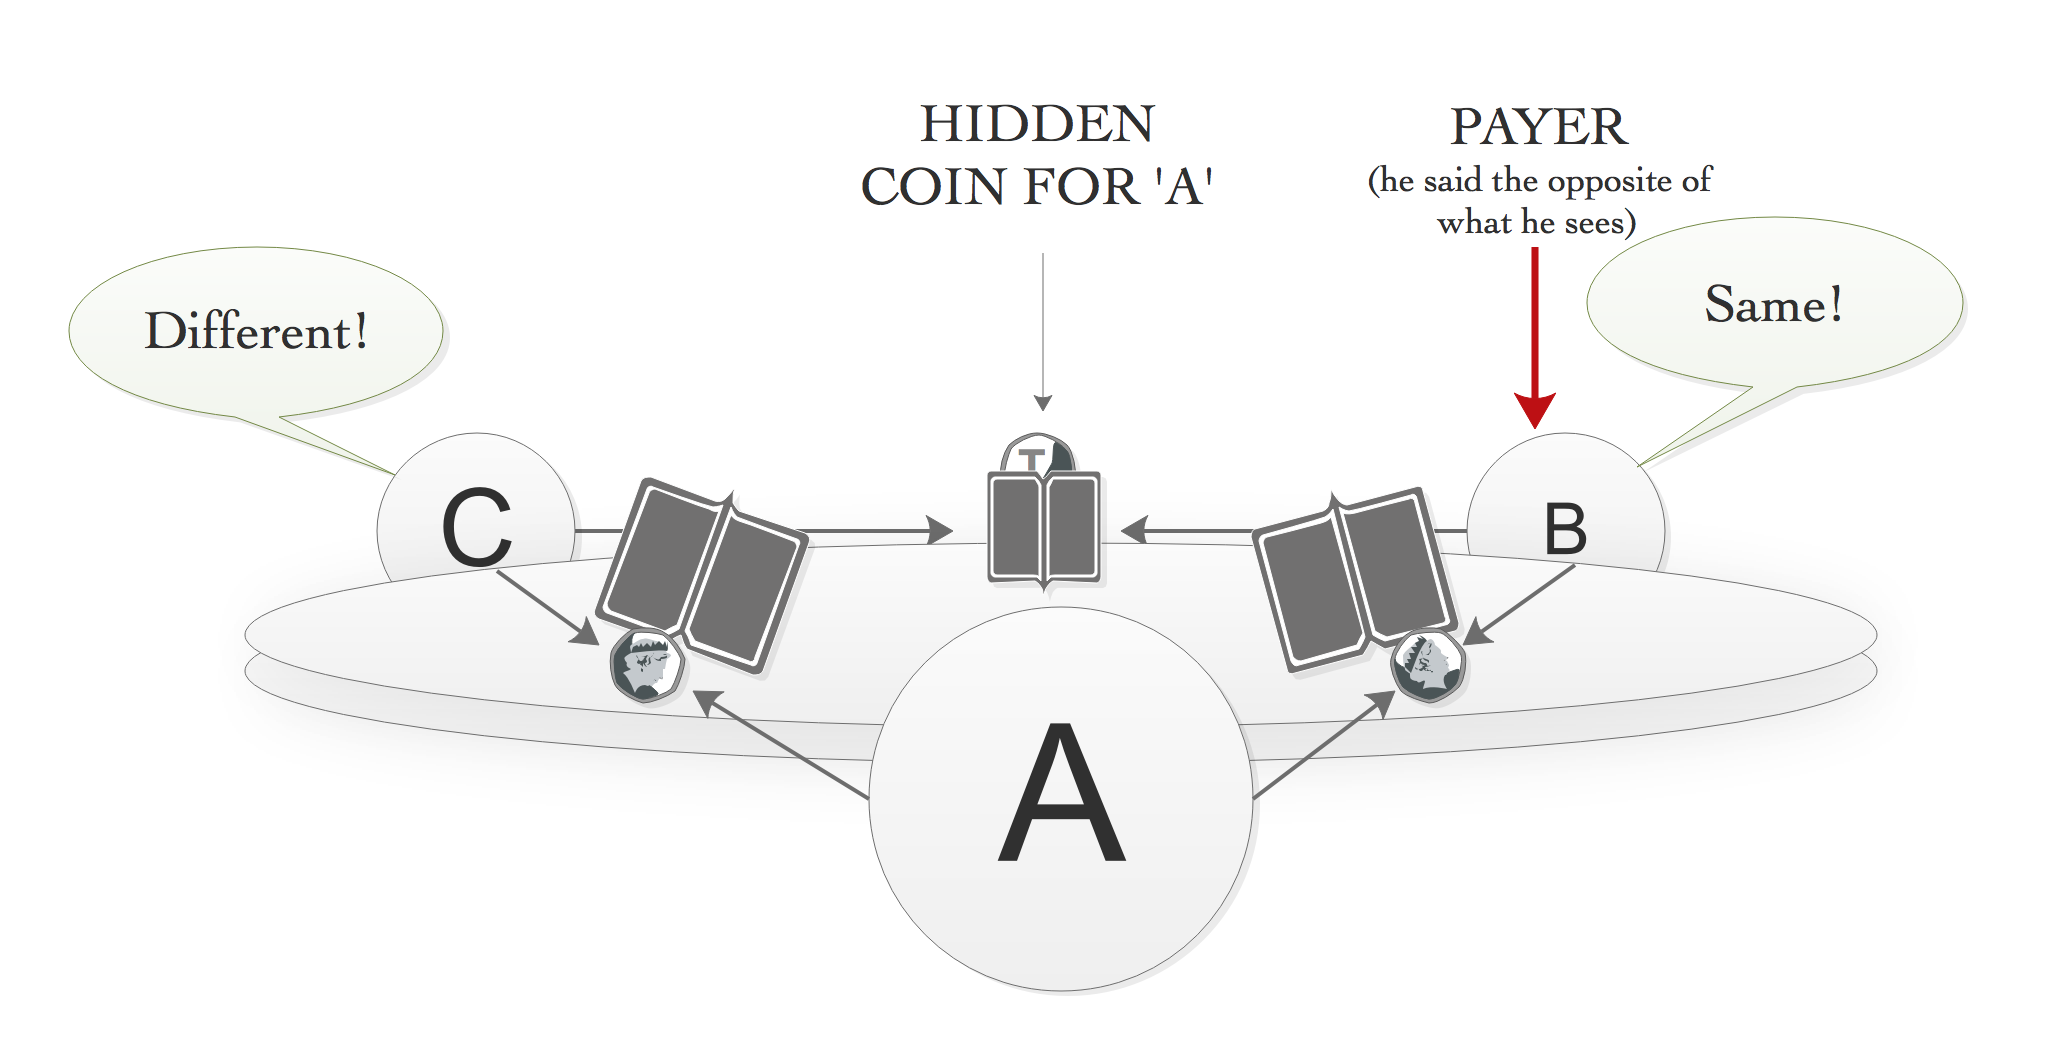
\includegraphics[width=0.80\textwidth]{Images/AsameCase2.png}
            \caption{Hidden Coin different from what A sees. B is the Payer.}
            \label{fig:AsameCaseDifferent}
        \end{figure}
        \item subject A sees two different coins (1 head and 1 tail). Then, if both the other cryptographers say 'Different', the payer is the one closest to the coin that A sees that is the same as the hidden coin (Figure \ref{fig:AdifferentCaseDifferent}); if both cryptographers say 'Same', the payer is the one closest to the coin that A sees that is different from the hidden coin (Figure \ref{fig:AdifferentCaseSame}) \cite{Chaum};
        \begin{figure}[h!]
            \centering
            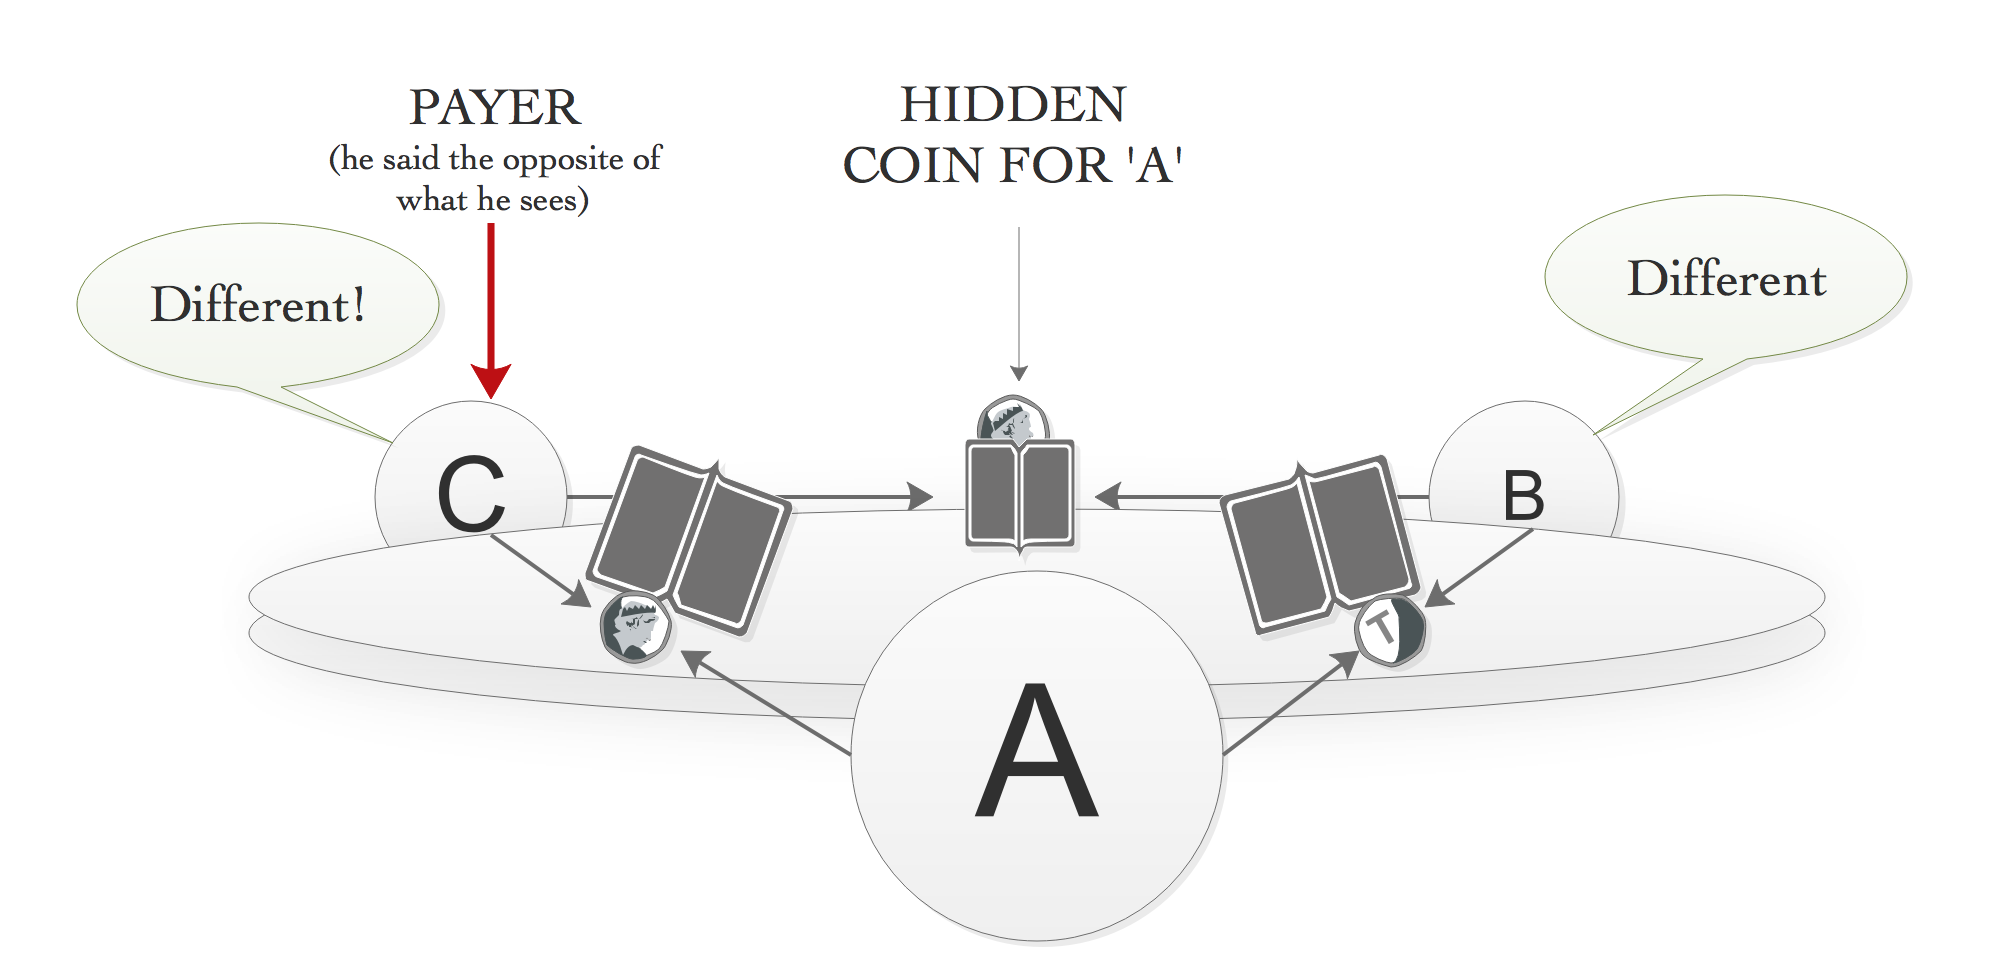
\includegraphics[width=0.80\textwidth]{Images/AdifferentCaseDifferent.png}
            \caption{Both Cryptographers say 'Different'. C is Payer.}
            \label{fig:AdifferentCaseDifferent}
        \end{figure}
        \begin{figure}[h!]
            \centering
            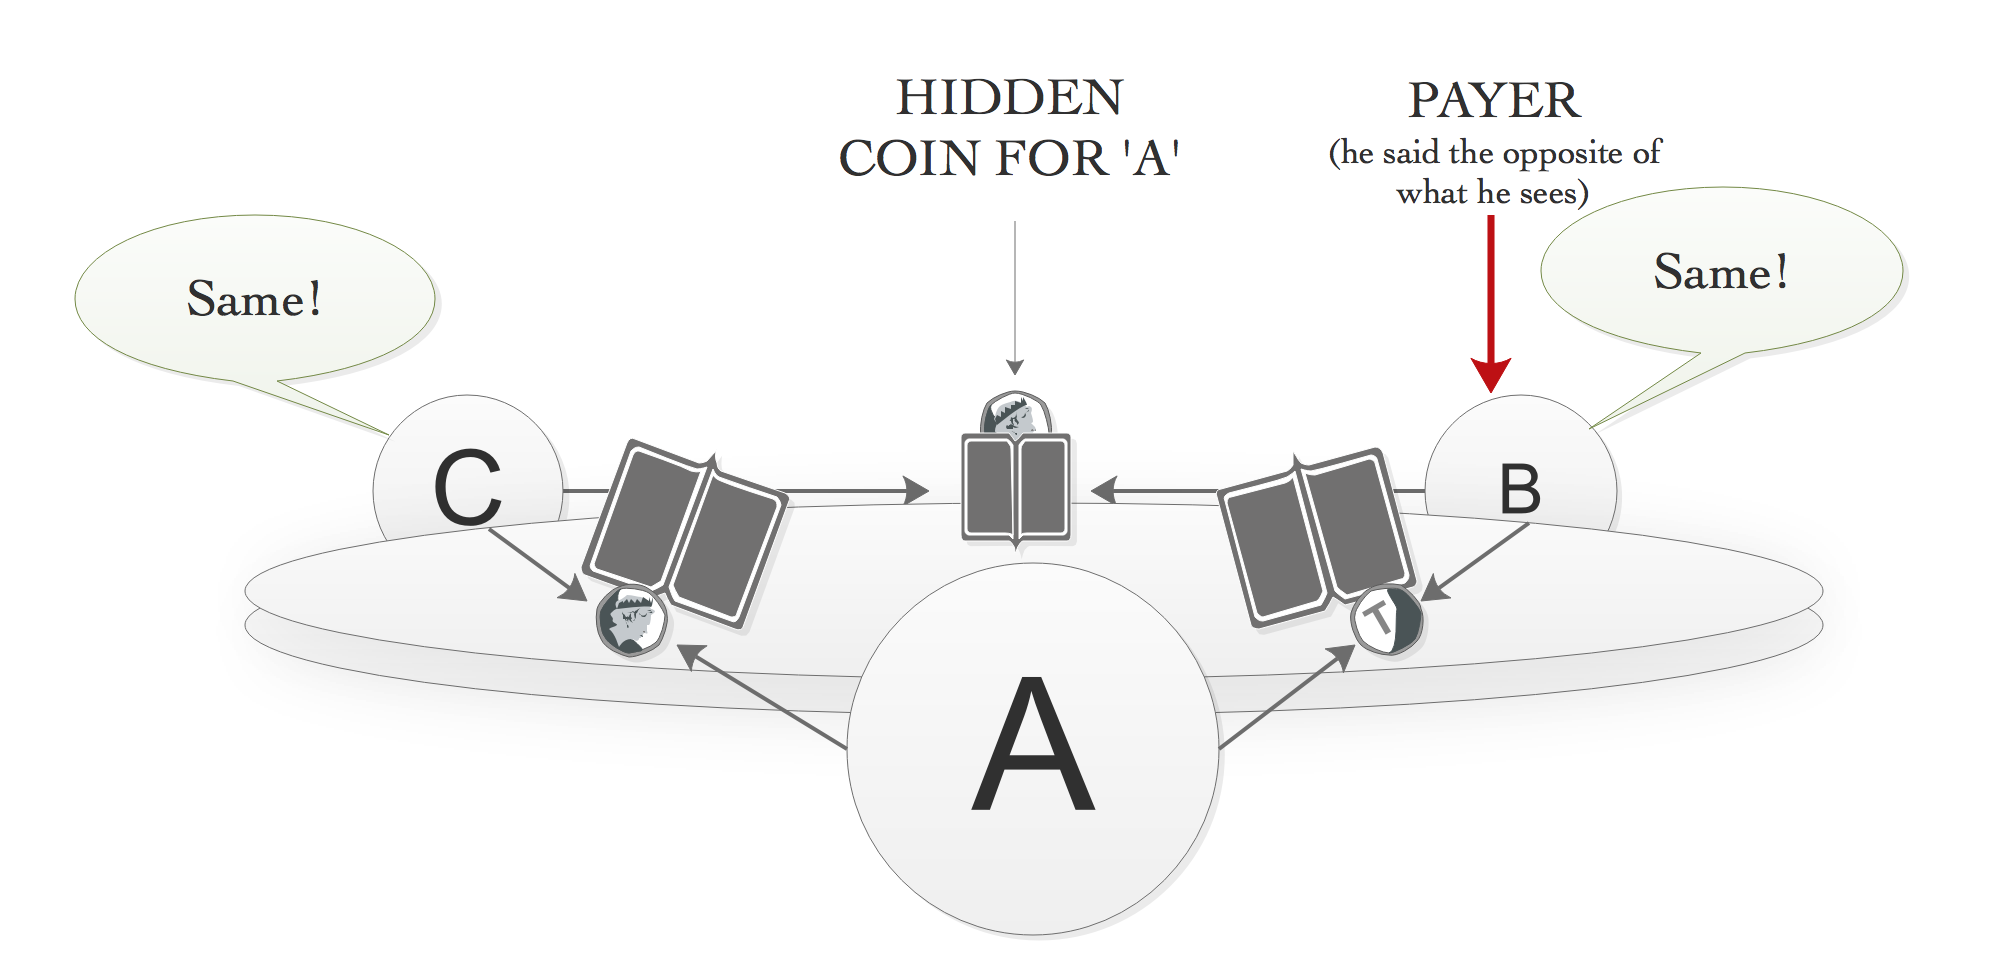
\includegraphics[width=0.80\textwidth]{Images/AdifferentCaseSame.png}
            \caption{Both Cryptographers say 'Same'. B is the Payer.}
            \label{fig:AdifferentCaseSame}
        \end{figure}
    \end{enumerate}
\end{enumerate}


As demonstrated in the scenarios above, the minimum number of participants required to carry out this protocol is three. If only two participants were present, sender anonymity would be guaranteed only in respect to an external observer of the network but not internally. Moreover, since the coin is unbiased, both head or tail have a 50{\%} likelihood of being the result. With such probability, a non-payer cryptographer can only guess the outcome of the hidden coin. Therefore, Chaum's protocol is unconditionally secure. \label{sec:internalExternalAnon}



\subsection{A Formal Exposition of the Protocol}
The analogy above has the purpose of facilitating the more formal exposition of the DC-Net protocol, which we present below. 

The Dining Cryptographers can be represented in graph theory, where each cryptographer is shown as a vertex. The flip coin presented in the analogy corresponds to a key exchange in a formal protocol. This key exchange is represented as an edge between two vertices, i.e. cryptographers. 

The basic version of the protocol uses one-bit keys. Therefore, only two values are possible, since a single bit can either be a 1 or a 0. From the metaphor of the coin, the head corresponds to a 1 and a tail is a 0 or vice versa.
The action of 'paying the dinner' corresponds to a participant, ergo a vertex, reversing his outcome before the broadcast. The action of 'announcing the result out loud' is a message broadcasted in the network. Lastly, each anonymous dinner payment is equivalent to a round of communication in which a node may broadcast a message.

\subsubsection{Exclusive OR (XOR)}
The operations executed by each cryptographer in stage 2 (see section \ref{sec:protocolStages}) to combine the results of different key-exchanges is done through the utilization of a logic operation called \textit{exclusive disjunction} or \textit{XOR}. The logical operation outputs true only if the the input values are different (table \ref{table:XOR}). The symbol of this operation is "$\oplus$".

\begin{table}[h!]
\centering
\caption{XOR Truth Table}
~\\[0.5ex]
\begin{tabular}{|| c | c | c ||} 
 \hline
 X & Y &  $X \oplus Y$ \\ [0.ex] 
 \hline\hline
 0 & 0 & 0 \\ 
 0 & 1 & 1 \\
 1 & 0 & 1 \\
 1 & 1 & 0 \\ [1ex]
 \hline
\end{tabular}
\label{table:XOR}
\end{table}

The XOR operation is also executed to combine the result of each vertex, i.e. cryptographer, at the third stage of the protocol, where at least three bits are present - one for each cryptographer in the network (see section \ref{sec:protocolStages}). In this case, the overall operation can be seen as a cascade of XOR operations between two input at a time (table \ref{table:XORextended}).


\begin{table}[h!]
\centering
\caption{XOR Truth Table with multiple values}
~\\[0.5ex]
\begin{tabular}{|| c | c | c | c ||} 
 \hline
 X & Y & Z & $(X \oplus Y) \oplus Z$ \\ [0.ex] 
 \hline\hline
 0 & 0 & 0 & 0 \\ 
 0 & 0 & 1 & 1 \\
 0 & 1 & 0 & 1 \\
 0 & 1 & 1 & 0 \\
 1 & 0 & 0 & 1 \\
 1 & 0 & 1 & 0 \\
 1 & 1 & 0 & 0 \\ 
 1 & 1 & 1 & 1 \\ [1ex]
 \hline
\end{tabular}
\label{table:XORextended}
\end{table}

The mathematical properties of the XOR operation are also very relevant for DC-Net problem \cite{Lewin} and are four:
\begin{enumerate} \label{sec:XORproperties} \label{sec:xorproperties}
    \item \textit{Commutative:} It does not matter the order of the inputs. $A \oplus B = B \oplus A$
    \item \textit{Associative:} XOR operation can be chained in any order $A \oplus (B \oplus C) = (A \oplus B) \oplus C$
    \item \textit{Identity Element:} XORing a value with zero will not change the value. $A \oplus 0 = A$
    \item \textit{Self-Inverse:} Any value XOR'd twice will cancel itself. In other words, a value XOR's with itself is equal zero. $A \oplus A = 0$
\end{enumerate}

\subsubsection{Exchange of one-bit messages with \textit{3} participants}
The following is the scenario and procedure of the protocol executed with the minimum number of three participants and expressed with a more formal notation (examples in figure \ref{fig:dcFormalnoMessage} and \ref{fig:dcFormalWithMessage}) :
\begin{enumerate}
    \item There are 3 vertices \textit{$P_1, P_2, P_3$};
    \item Each vertex is part of two adjacencies, one for each neighbour. For example, vertex \textit{$P_1$} is part belongs to \textit{$N(P_1,P_2)$} and \textit{$N(P_1, P_3)$};
    \item Each adjacency is also an edge that represents a key. \textit{$P_1$} will have edges \textit{$K_{1,2}$} and \textit{$K_{1,3}$};
    \item Each vertex will calculate the value to be broadcasted. In the example of \textit{$P_1$}: 
    \begin{enumerate}
        \item If P1 does not want to send a message ($M_1$), \textit{$M_1 = K_{1,2} \oplus K_{1,3} \oplus 0 $}. This is equivalent to \textit{$M_1 = K_{1,2} \oplus K_{1,3}$};
        \item If P1 wants to send a message ($M_1$) \textit{$M_1 = K_{1,2} \oplus K_{1,3} \oplus 1 $}. This is equivalent to \textit{$M_1 = \neg(K_{1,2} \oplus K_{1,3}) $};
    \end{enumerate}
    \item The final round result (R) will be calculated by XORing all the results such that \textit{$R = M_1 \oplus M_2 \oplus M_3$}.
\end{enumerate}


\begin{figure}[h!]
    \centering
    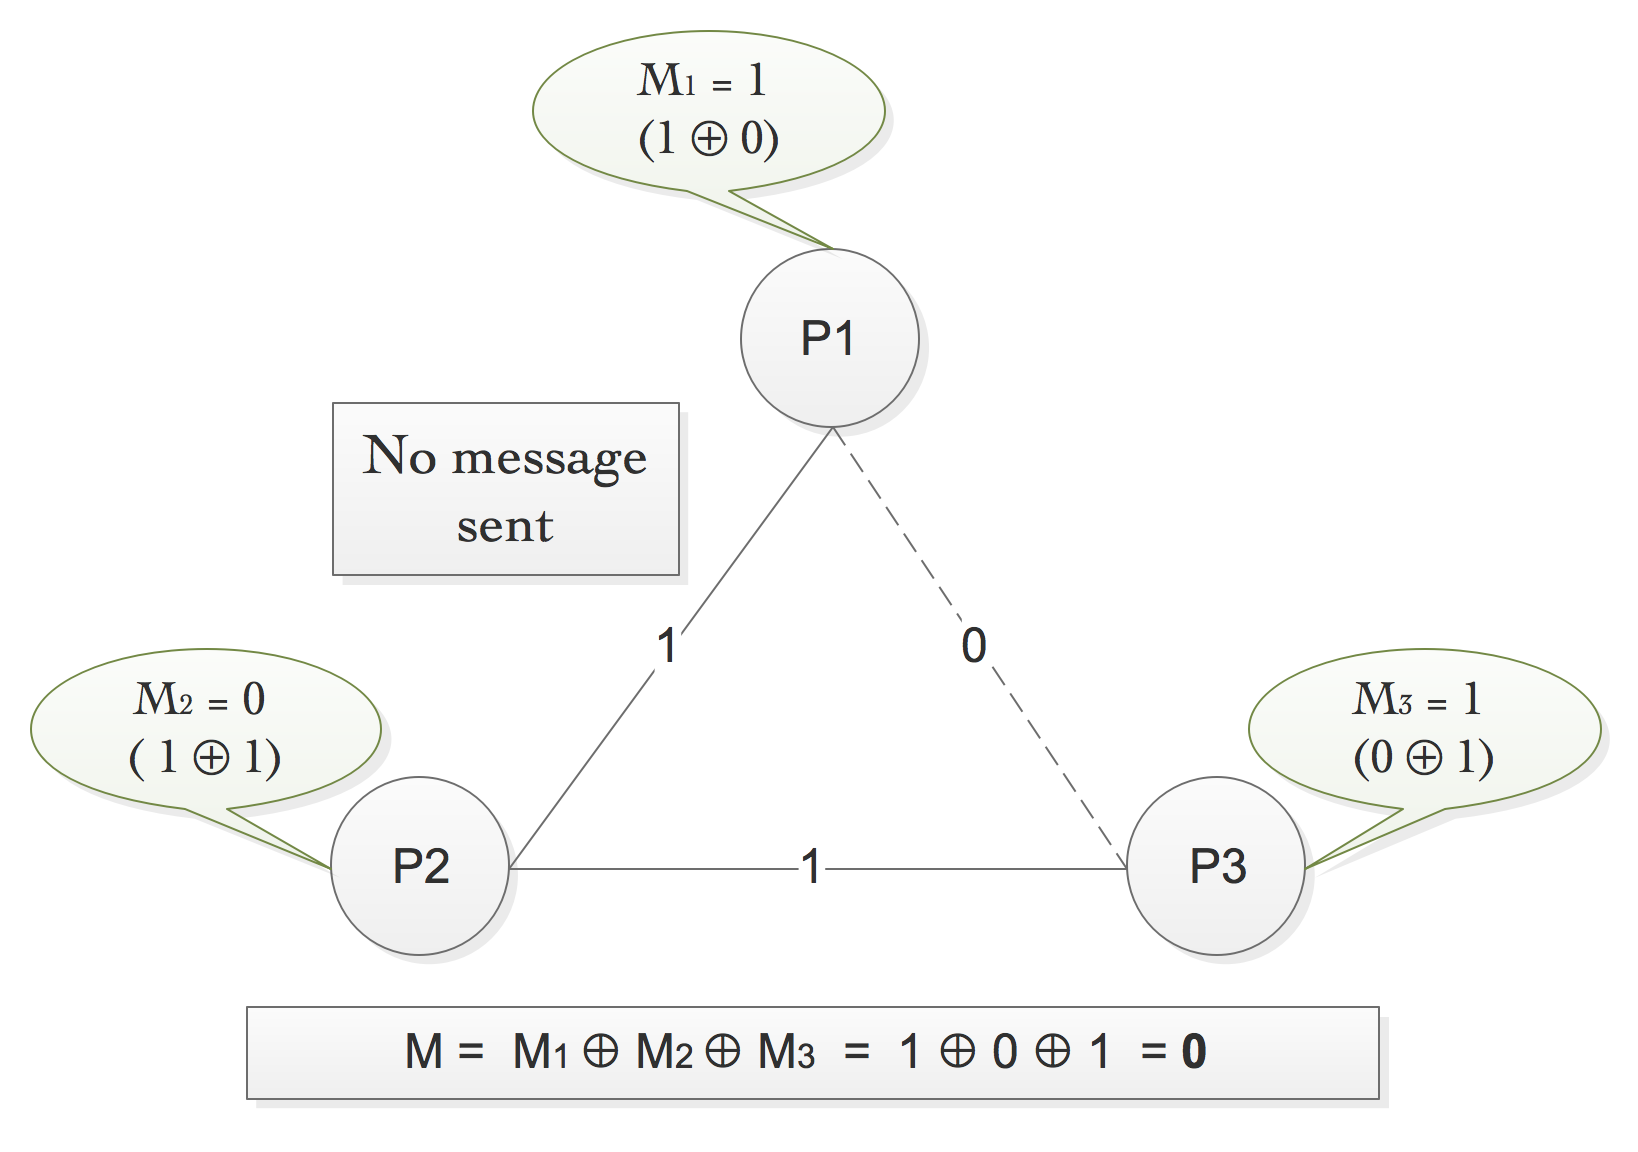
\includegraphics[width=0.70\textwidth]{Images/DCFormalNoMessage.png}
    \caption{3 vertices message exchange with no message sent (even number of 1s)}
    \label{fig:dcFormalnoMessage}
\end{figure}

\begin{figure}[h!]
    \centering
    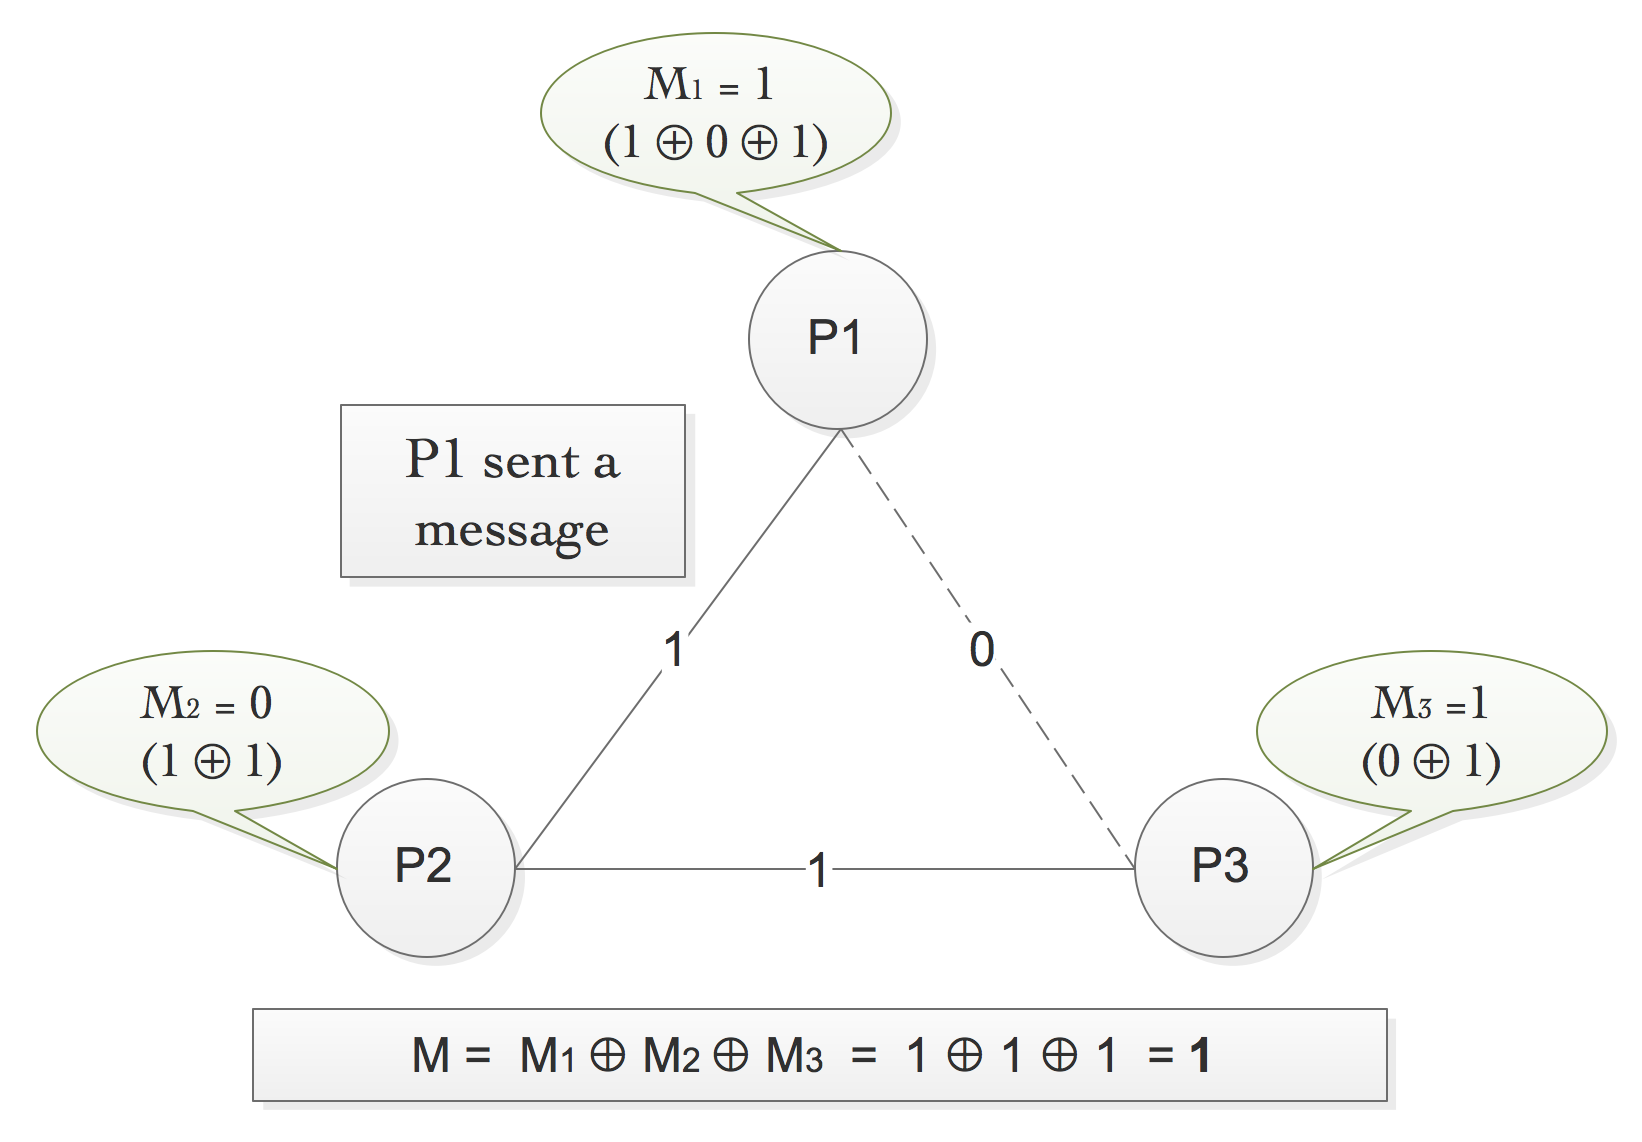
\includegraphics[width=0.70\textwidth]{Images/DCFormalWithMessage.png}
    \caption{3 vertices message exchange with a message sender (odd number of 1s)}
    \label{fig:dcFormalWithMessage}
\end{figure}

From now on, the dinner analogy language and the formal graph notation will be used interchangeably. \newline \newline \newline

\section{Limitations} \label{sec:limitations}
As already mentioned, the Dining Cryptographer is a very effective protocol to guarantee sender anonymity in \textit{theory}. In reality, there are some limitations, which affect the practicality of the protocol in a real-world use to the point there does not exist a fully-working version of this protocol.
The three main limitations we now turn to explore are: message collision, communication disruption and communication overhead. 

\subsection{Collisions}
A message collision is the attempt of two cryptographers to send a message in the same round of communication.So far, one of the assumptions to verify the correctness and efficacy of the protocol was that only one vertex, or cryptographer, broadcasts a message per round. However, it is possible and likely that multiple vertices will try to send a message, i.e. a reversed response, in the same round, which leads to a message collision. The consequence is that, if an even number cryptographers sends a message in the same round, the final result will be 0, which equates to 'no one has flipped their message'. If an odd number of cryptographers sends a message in the same round, the final result will be 1, which corresponds to just one cryptographer having sent a message.
Therefore, if this probable scenario is not acknowledged, the correctness of the protocol is jeopardized.

\subsection{Disruption and Collusion} \label{sec:disruptionlimitation}
Disruption and collusion are two limitations brought by the presence of active attackers in the network. A passive attacker is a principal that can only intercepts messages being exchanged, eavesdropper. An active attacker, on the other hand, performs malicious actions, such changing the content of a messages before sending it. The protocol is secure in respect to an eavesdropper. However, a cryptographer inside the network, who is an active attacker, could inject falsified responses instead of following the protocol rules. Unless these forged messages are somehow detected, this can easily disrupt the execution of the protocol.

Another possible problem may be incurred by an active attacker delaying his responses at each round. Since the final result of the round cannot be calculated unless all the clients have provided their responses, such delay may affect the availability of the service \cite{Fischer}.

Moreover, active attackers within the network may collaborate to uncover the real sender of a message by pooling together their keys. This possible threat is called collusion. Assuming three participants in the network and one cryptographer discovering the value of the third hidden coin via key pooling with one of his neighbours, this malicious cryptographer can establish who sender is, if any is present \cite{Chaum}. 

This type of collaboration is treated in more depth by other information security academics, such as Waidner \cite{Waidner} or Safavi-Naini and Susilo \cite{Susilo}. As established by several academic analyses, the technical capability of colluding also depends on the key-sharing topology implemented, therefore this limitation may be mitigated by using specific architectures (see section \ref{sec:participantsextention}). 


\subsection{Communication Overhead} \label{sec:complexitylimitation}
An overhead is an excess of computation power or resources needed to perform a specific task. 

Depending on the architecture implemented, there are several messages to be sent in order to hide the real sender. Each client is part of two messages per round of communication: one message sent as part of the sender anonymity set and one message is received as part of the recipient anonymity set.

In the key-sharing graph explained so far (see section \ref{sec:ringtopology}), given $n$ participants, a single bit message will require at least $2n$ messages to be sent on the network in a single round. 

In another architecture presented later in section \ref{sec:fullmeshtopology}, each client broadcasts $n-1$ messages, leading to $2(n * (n - 1))$ exchanges per round.

This overhead is necessary to guarantee anonymity and the larger the $n$ the higher the level of anonymity, as seen in section \ref{sec:anonymityset}. 

The operating cost is likely to be the main reasons why such powerful protocol is deemed impractical \cite{Scholz}.


\section{Extensions of Basic Protocol}

The basic protocol is presented with specific message length (one-bit messages) and a given number of participants (three). However, in the real world, it is highly unlikely that a network would exhibit three participants exchanging only one-bit messages. Based on such features, the pertinence of the protocol is restricted to an unrealistic scenario. 

To extend the applicability of Chaum's protocol, we can consider more participants and more complex messages within the network as per below.

\subsection{Increase number of participants} \label{sec:participantsextention}
The basic protocol can be generalized to accommodate \textit{n} participants (more than 3) with two different topologies.

\subsubsection{Ring Topology} \label{sec:ringtopology}
One of the two methods to extend the protocol to multiple payers is very similar to the one presented up to this point. Each vertex will have only two edges, one with each neighbour, and the protocol follows the same rules, as showed in figure \ref{fig:nparticipants1}.

More formally speaking: 
\begin{enumerate}
    \item There are \textit{n} vertices named \textit{$P_1, P_2, ..., P_n$};
    \item Each vertex \textit{$P_i$} is part of two adjacencies, one for each neighbour: \textit{$N(P_i,P_{i-1}), N(P_i, P_{i+1})$};
    \item Each adjacency is also an edge that represents a key: \textit{$K_{i,i-1}$} and \textit{$K_{i,i+1}$};
    \item Each vertex will calculate the value to be broadcasted as follows: \begin{enumerate}
        \item If the node does not want to send a message \textit{$M_i = K_{i,i-1} \oplus K_{i,i+1} \oplus 0 $}. This is equivalent to \textit{$M = K_{i,i-1} \oplus K_{i,i+1}$};
        \item If the node wants to send a message \textit{$M_i = K_{i,i-1} \oplus K_{i,i+1} \oplus 1 $}. This is equivalent to \textit{$M_i = \neg(K_{i,i-1} \oplus K_{i,i+1}) $};
    \end{enumerate}
    \item The final round result will be calculated by XORing all the results such that \textit{$R = M_1 \oplus M_2 \oplus ... \oplus M_n$} (example in figure \ref{fig:nparticipants1}).
\end{enumerate}


\begin{figure}[h!]
    \centering
    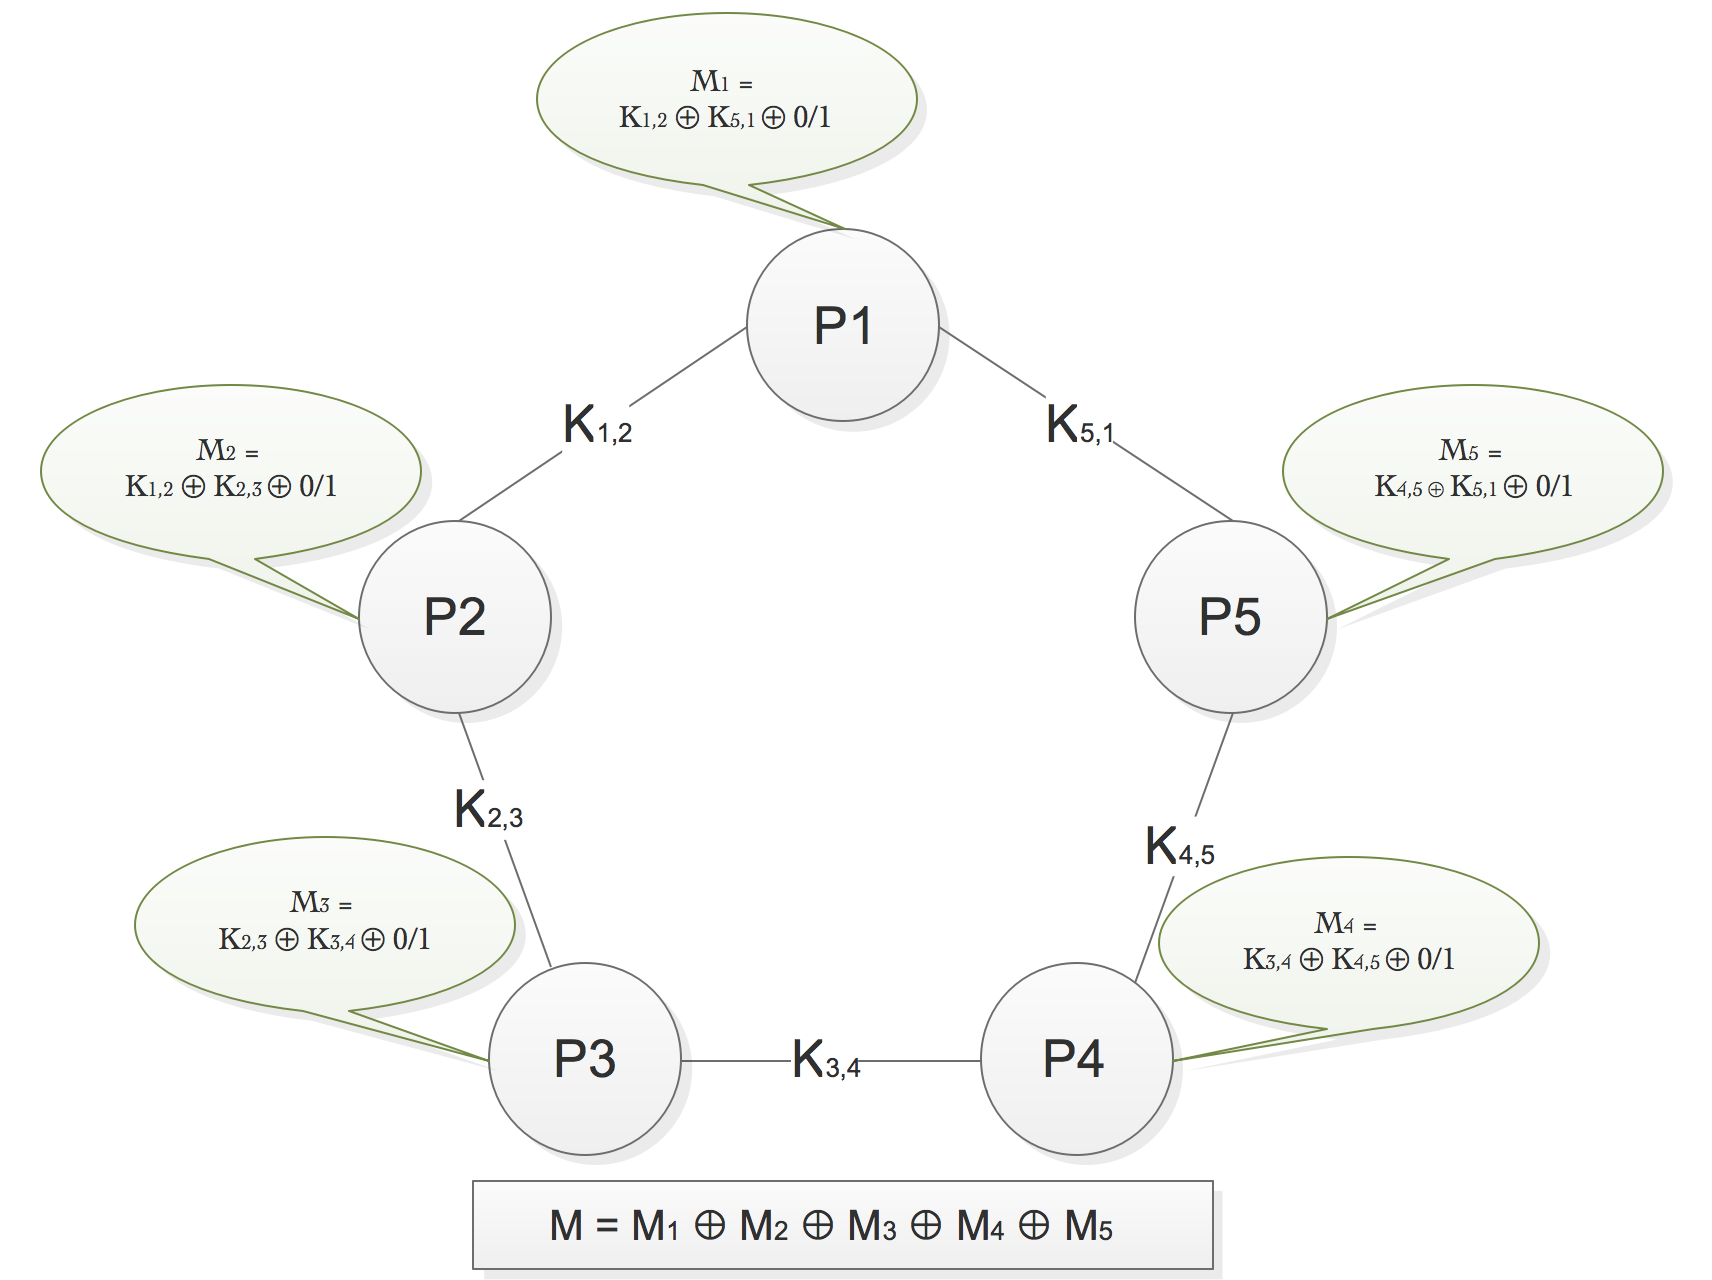
\includegraphics[width=0.95\textwidth]{Images/nparticipants1.png}
    \caption{Message exchange of 5 participants with ring topology}
    \label{fig:nparticipants1}
\end{figure}


\subsubsection{Full Mesh Topology} \label{sec:fullmeshtopology}
The second approach, presented by Chaum, differs in the respect that each vertex has an edge connecting with every other vertex \cite{Chaum}. Therefore, whichever pair of cryptographers, no matter if they are adjacent or not, shares a secret key. In such scenario, each vertex holds \textit{$n - 1$} keys, and his response will be the result of XORing all these values. The message a cryptographer sends is flipped, hence XORed with 1, if he  wishes to send a message.

More formally speaking:
\begin{enumerate}
    \item There are \textit{n} vertices named \textit{$P_1, P_2, ..., P_n$};
    \item Each vertex has \textit{$n-1$} edges that represent the same number of keys key: \textit{$K_{i,i-1}, K_{i,i+1}, ... , K_{i,n} $} (excluding \textit{$K_{i,i}$});
    \item Each vertex will calculate the value to be broadcasted \textit{$M_i = K_{i,i-1} \oplus K_{i,i+1} \oplus ... \oplus K_{P_i,P_n} $}. \textit{M} will be reversed if \textit{$P_i$} wants to broadcast his 1 bit message.
    \item The final round result will be calculated by XORing all the results such that \textit{$R = M_1 \oplus M_2 \oplus ... \oplus M_n$} (Example in figure \ref{fig:nparticipants2}). \newline
\end{enumerate}


\begin{figure}[h!]
    \centering
    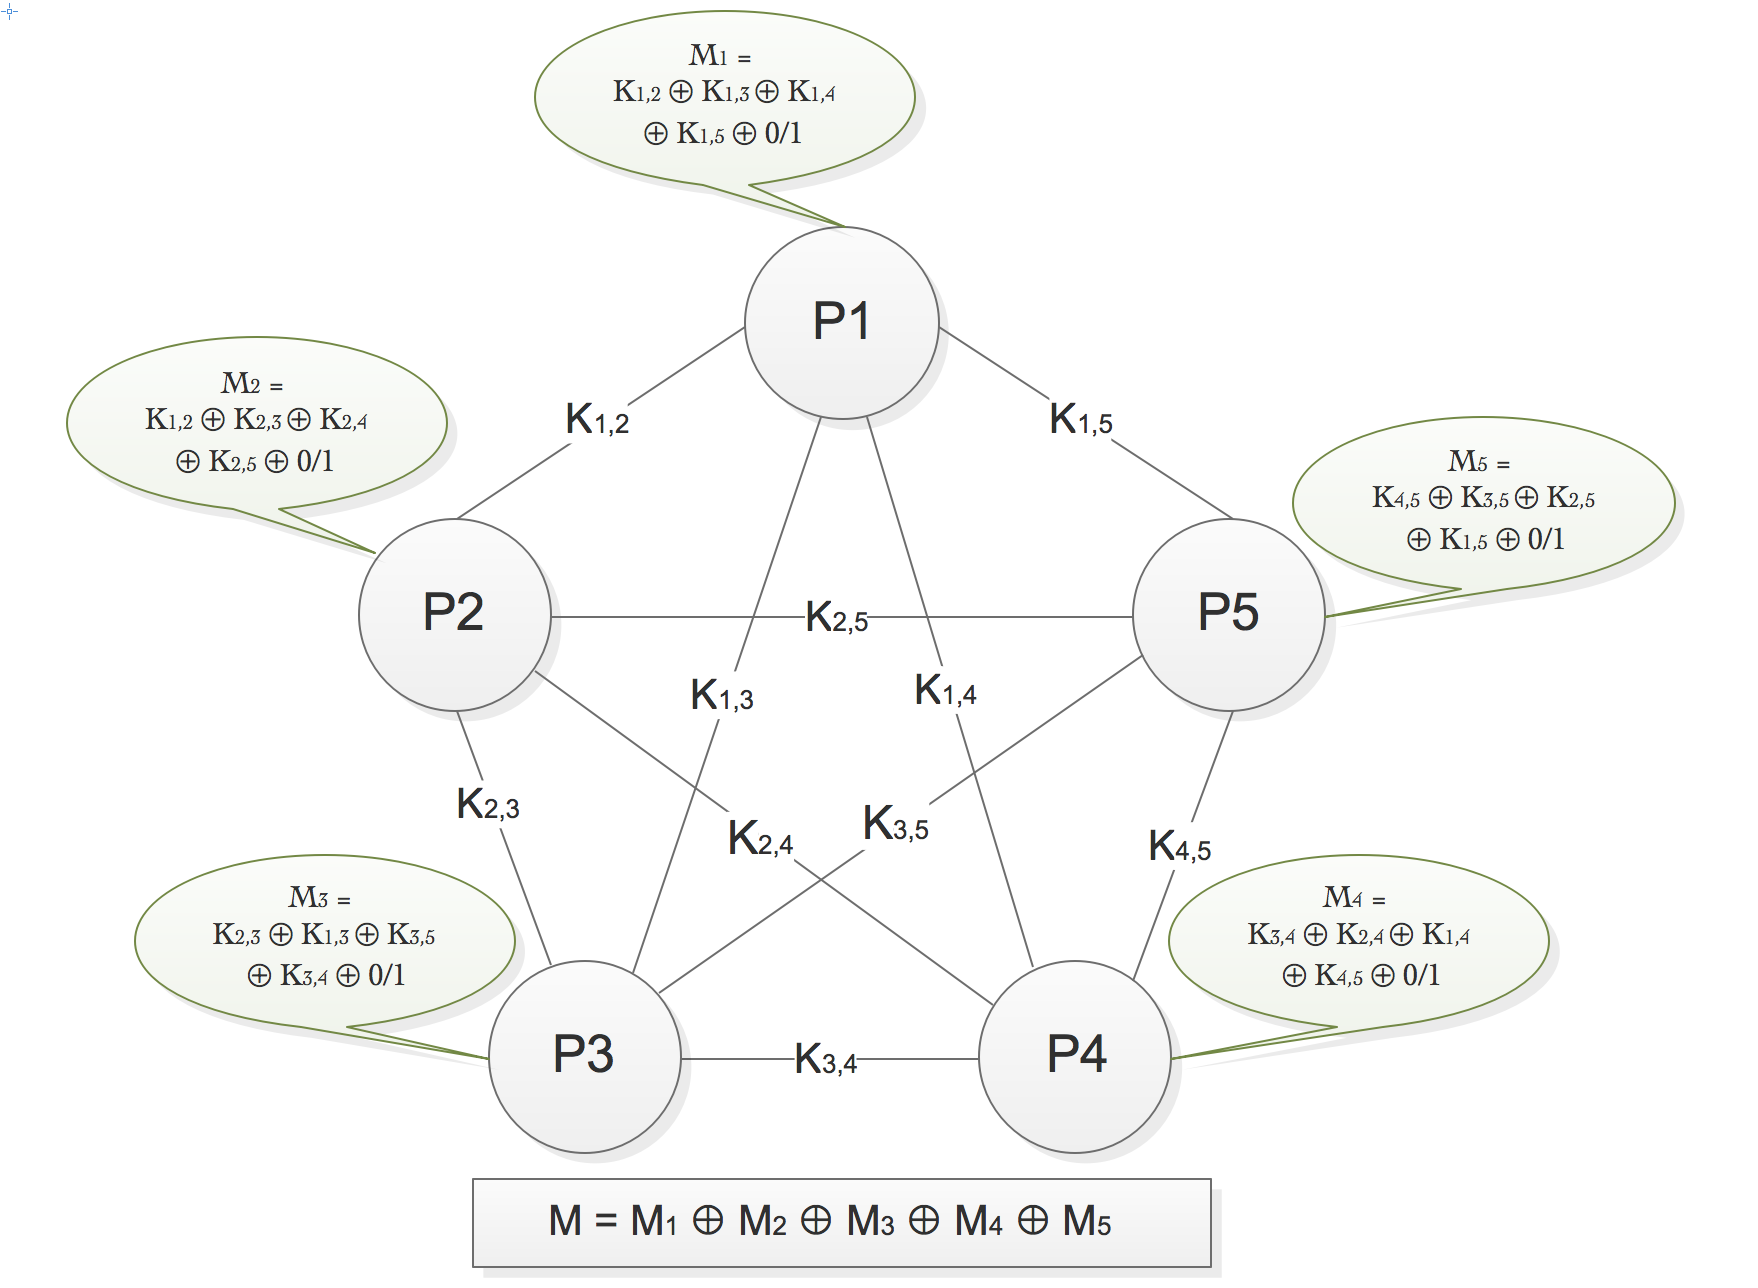
\includegraphics[width=0.95\textwidth]{Images/nparticipants2.png}
    \caption{Message exchange of 5 participants with full-mesh topology}
    \label{fig:nparticipants2}
\end{figure}


Each approach presents advantages over the other. A ring topology uses less computational power therefore presents less overhead, as explained in section \ref{sec:complexitylimitation}, while a full-mesh topology can be considered more secure against collusion of participants, explained in section \ref{sec:disruptionlimitation}.
The overall benefit of multiple participants within a network is twofold:
\begin{enumerate}
    \item adapting the protocol to a real-world scenario as it is unreasonable to have a network with only three nodes;
    \item growing the number of participants increases the level on anonymity as explained in section \ref{sec:anonymityset}; \newline \newline
\end{enumerate} 

\subsection{Extend message length}

Accommodating many participants makes the protocol more suitable for a real application. So does the possibility of sending longer messages. Increasing the length of messages to more than one bit may have two possible meanings: (1) to send different keys that are longer than one bit or (2) to repeat the round multiple times in order to gather pieces of the same message.

\subsubsection{Keys longer than one bit} \label{sec:longerKeys}
The range of possible keys can be incremented by growing the number of bits in a key. If the keys are, for example, 8-bit long, the possible randomly generated value of a key can be anything between 0 and 255 ($2^8$), as opposed to a 1-bit key where values can only be 0 or 1 ($2^1$) \cite{Scholz}. A 1-bit key network allows a sender cryptographer to XOR his two secret keys with a 0 or 1, which corresponds to flipping a message (see section \ref{}). A 8-bit key network allows the sender cryptographer to XOR his two secret keys with a value, i.e. anonymous message, that can be anything between 0-255 as the range of the key. An example is provided in figure \ref{fig:xorlongkeys}.

\begin{figure}[h!]
    \centering
    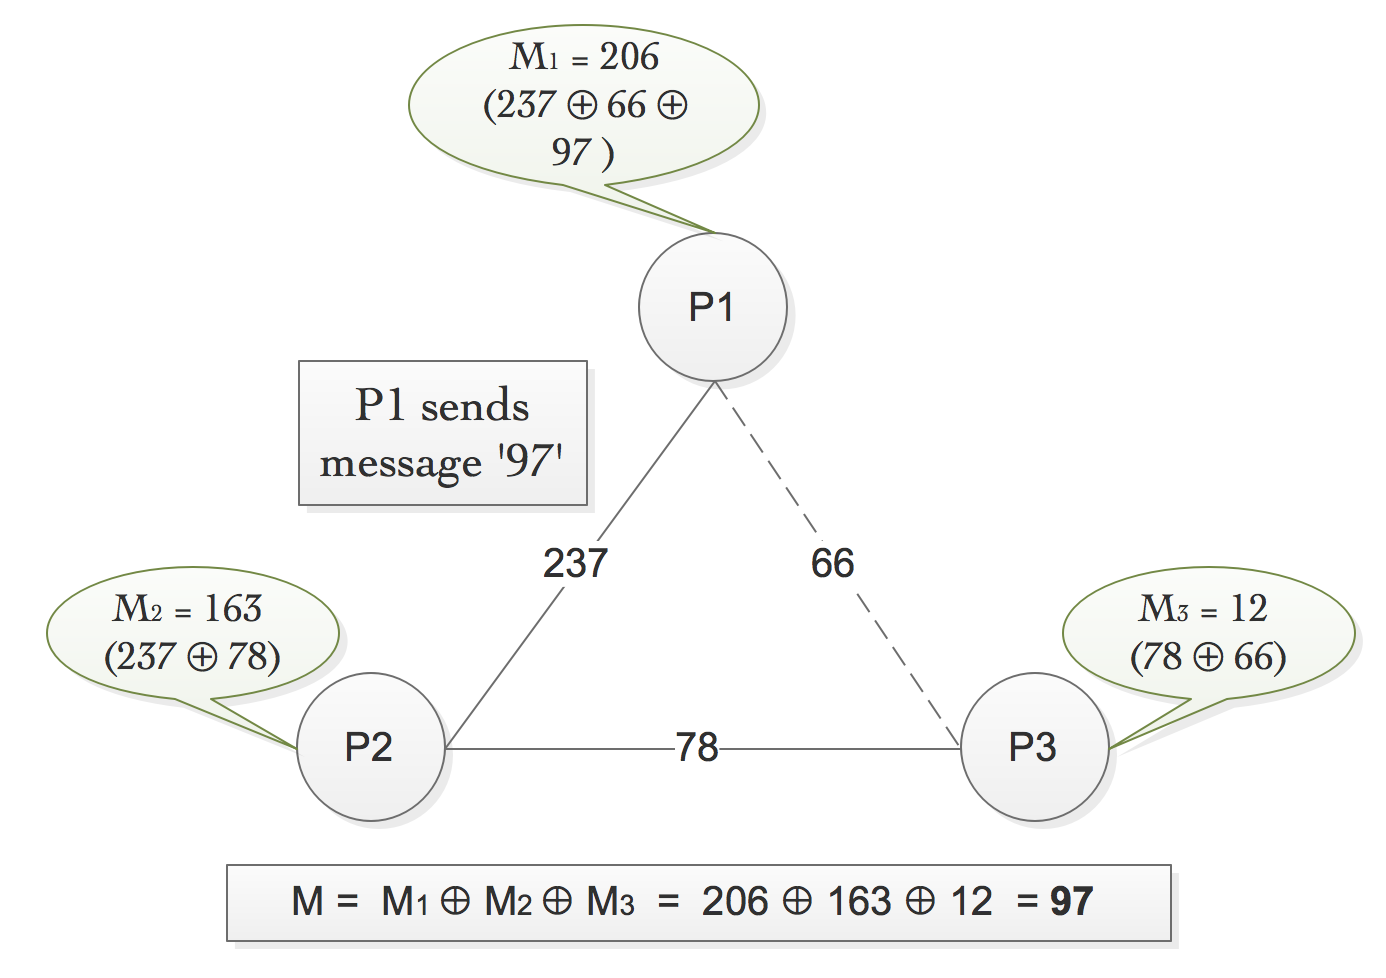
\includegraphics[width=0.95\textwidth]{Images/dcnet8bitkeys.png}
    \caption{Three participants round with 8-bit keys}
    \label{fig:xorlongkeys}
\end{figure}

Adopting longer keys can be useful. Take, for example, the ASCII character encoding, a technique to represent a character (e.g. a number, symbols or letters) has a corresponding number. The official ASCII encoding contains 128 characters, and the extended version has 256 of them, which can therefore represented in 8 bits ($2^8$). Therefore, a cryptographer wanting to send a specific letter may simply XOR his two secret keys with the ASCII number that represents the said letter.


\subsubsection{Multiple Rounds} \label{sec:messageExtentionRounds}
An alternative to sending longer messages is to repeat the protocol multiple times. The repetition allows a node to send multiple messages in a row, either with a 1-bit key or in conjunction with the long-key technique explained in the previous section. By repeating the protocol multiple rounds, a cryptographer can broadcast a cumulative message that might be more meaningful that a single round of communication.



\section{Practical Considerations}
As we have discussed, the Dining Cryptographers protocol tries to jointly compute the result of a function from different nodes. Such type of protocol is a specific sub-field of cryptography called 'secure multi-party computation' \cite{wiki1}. 

The fact that nodes do not reside in the same physical location, adds further complications to the scenario, such as the network topology used to implement the protocol, the implications of the distributed architecture over the protocol's computation and the method of transmission of the secret one-time keys  to each node.

(What network topology is it used to implement this protocol? 

What implication has the distributed architecture over the protocol computation? 

As DC-Net relies on confidential one-time keys, how does such secret reach each node?)

\noindent \newline These practical issues are addressed in this section to start considering what are the repercussions of implementing a protocol that, in theory, provides flawless sender anonymity.


\subsection{Key Exchange Channels} \label{sec:keyExchangeMethods}
A fundamental problem in cryptography to ensure the effectiveness of a protocol is how to exchange keys securely. The DC-net is no exception: in order to guarantee the anonymity of the senders and recipient in the network, the single part of communication that needs to be securely completed is the exchange of the keys.

\subsubsection{Physical Disks}
In its original paper, Chaum proposes the exchange of physical optical disks that with today's storage capabilities can provide trillions of randomly-generated bits to be used as keys \cite{Chaum}. However, this is impractical for real-world applications, especially for large networks. 

\subsubsection{Synchronised Number Generators}
Another possibility is to use synchronised cryptographically secure pseudo-random number generators (CSPRNG). This entails that each client has its own generator and no key is ever transmitted on the network. Consequently, the reliability of the DC-net protocol would be based on the implementation of the generators \cite{Chaum}.

\subsubsection{Public-key Cryptography}
Lastly, a practical alternative is to use public-key cryptography. The most commonly used methods are \cite{Chaum}:
\begin{enumerate}
    \item RSA cryptosystem: employing a pair of private and public key for each client in order to encrypt keys securely;
    \item Diffie-Hellman 'key-exchange': a key generation protocol that can work on completely insecure communication channels to create keys for participants without ever transmitting it over the network \cite{Golle}.
\end{enumerate}


\subsection{Possible Network Topologies} \label{sec:networkTopologies}
There are two main network topologies that can be used in order to implement a DC-Net: peer-to-peer an client-server. The network topology is not to be confused with the key-exchange topologies presented in section \ref{sec:participantsextention}.

\subsubsection{Peer-to-Peer} \label{sec:peertopeer}
This topology resembles closely the description of the protocol so far, in which a node communicates directly with his neighbours or with all participants in the network. This setting requires nodes to handle the whole of the communication, key generation, and broadcast.
Peer-to-peer does not provide a mechanism to detect collisions efficiently, since each nodes cannot know if neighbours are sending their correct responses or if they are adding a message to their broadcast.


\subsubsection{Client-Server} \label{sec:clientserver}
A client-server topology decreases the responsibilities of a node given the presence of a centralized DC-net service. Plus, the server has a much more complete vision of the network in respect to a node. \emph{This is a very contradictory factor}. On one hand, it offers the DC-Net various capabilities such as detecting collisions efficiently, generating keys, helping the clients broadcast messages at the same time. On the other hand, it introduces issue of \emph{trust}. The clients are supposed to believe that the server is a non-malicious entity that will facilitate the communication. In addition, if someone has access to the server and this is the place where the keys are generated, the protocol would be completely compromised.

\subsection{Detecting Collisions}
The protocol's limitation of potential collisions is to be addressed in order to transmit useful messages. Without such feature the protocol would be secure but useless. \newline

A DC-Net implementation that does not possess a DC-net central entity to coordinate the network, the collisions would be detected only by the actual message senders. For example, in a one-bit key message exchange, if a node transmits a message and the final broadcast results in no one having sent a message, then the node can deduct the presence of an even number of message senders in this given round. To tackle this issue, the said node can retransmit after a random number of communications rounds. \newline

The above collision-detection technique is not effective in a scenario in which a node would like to send a long message across multiple rounds (section \ref{sec:messageExtentionRounds}). This instance demands for an uninterrupted flow of communication without collisions, otherwise the meaning of whole message can be considered affected.
In this scenario, the only possible solution is to employee a server as central DC-Net service. This entity would be aware of who the message sender is so as to reserve a number of rounds only for that given node.


\section{Existing DC-net simulation tools} \label{sec:similarWorks}
It is important to research the area of interest of a project in the early stages of a piece of work in order to understand the current state of the art, draw inspiration, and determine possible areas of improvement of the matter considered.

The Dining Cryptographers protocol is an extensively studied topic addressed by several academic papers. The basic idea proposed by Chaum contains a number of limitations as we have seen in section \ref{sec:limitations}, and various papers propose complex and interesting solutions to solve very specific issues of the protocol (e.g. how to exchange keys securely). The common denominator of all these works is that they are largely theoretical. 

The main purpose of this project is to develop a practical simulation tool for the Dining Cryptographers protocol, and therefore the research of similar works focuses purely on practical implementations and simulations of a DC-Net. As a matter of fact, the outcome of the research of existing tools is the leading motivation for implementing a DC-Net simulator. Namely, while there exists a wealth of academic papers that thoroughly examines the protocol on a theoretical level, there is an easily identifiable gap in the domain of practical software systems that exemplifies the functioning of this protocol.

In addition, the handful of projects found is of little help in deepening the understanding of the protocol since these simulations are mostly command-line tools that, beside the unhelpful user experience, are not well-documented on how to perform even a single round of communication. \newline

Given that  DC Networks are mostly a theoretical concept, researching the wide internet lead exclusively to academic papers. A more sensible approach to find possible implementations is to search through the development platform GitHub. Below are some implementation found, which highlight the shortcomings of the current state of art in DC-Net implementations.

\subsection{Example 1}
The first is a command line tool that presents extensive documentation, which appears to be very handy (figure \ref{fig:work1documentation}). However, all the commands listed in the documentation do not work, return errors, and there is no troubleshooting guide (figure \ref{fig:work1error}).

\begin{figure}[h!]
    \centering
    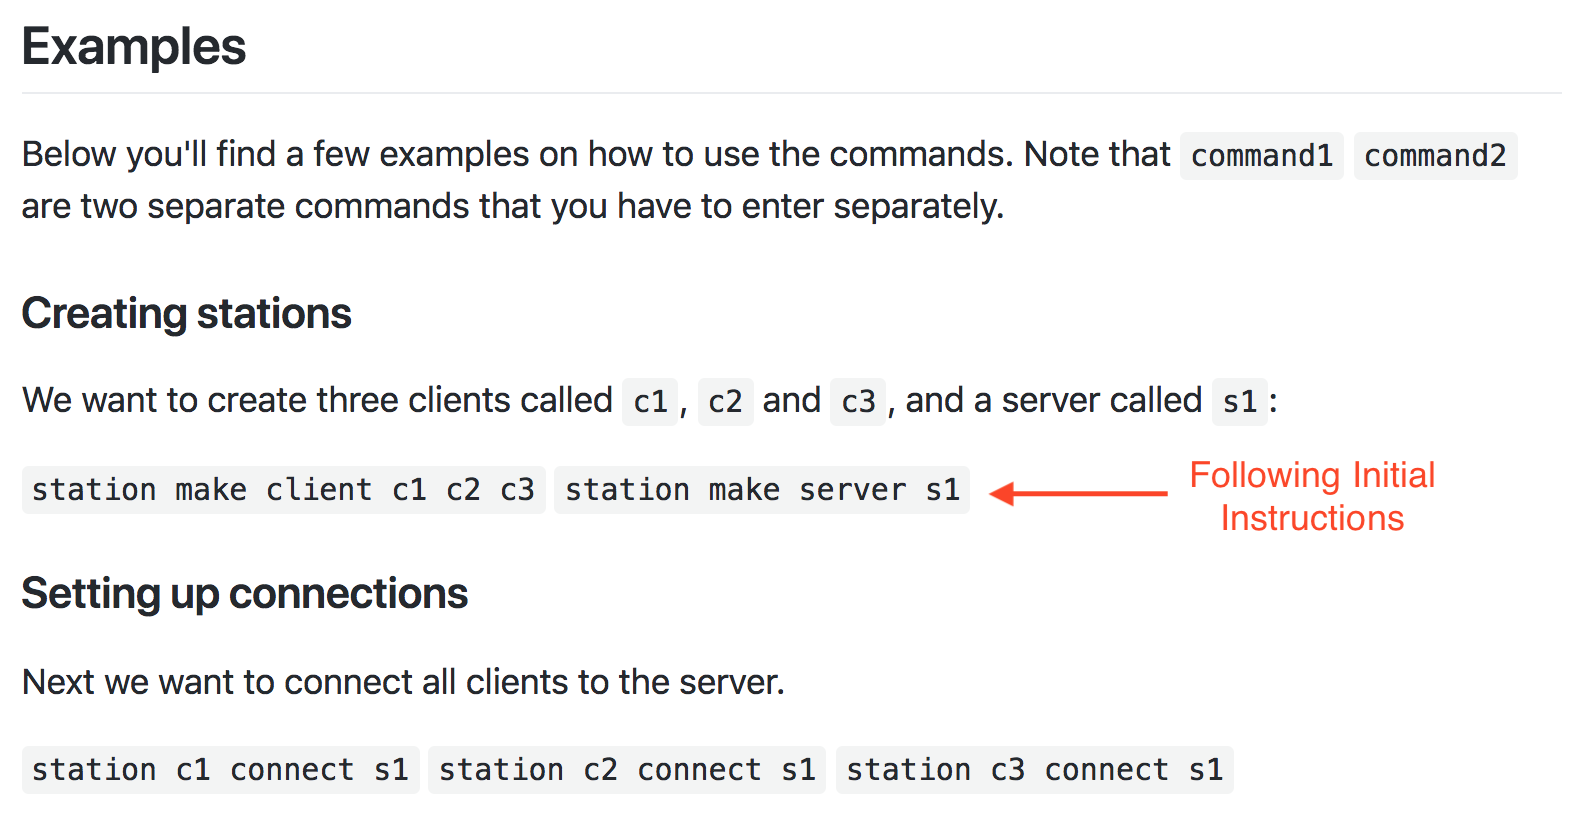
\includegraphics[width=0.7\textwidth]{Images/work1WellDocumented.png}
    \caption{Extensive encouraging documentation.}
    \label{fig:work1documentation}
\end{figure}

\begin{figure}[h!]
    \centering
    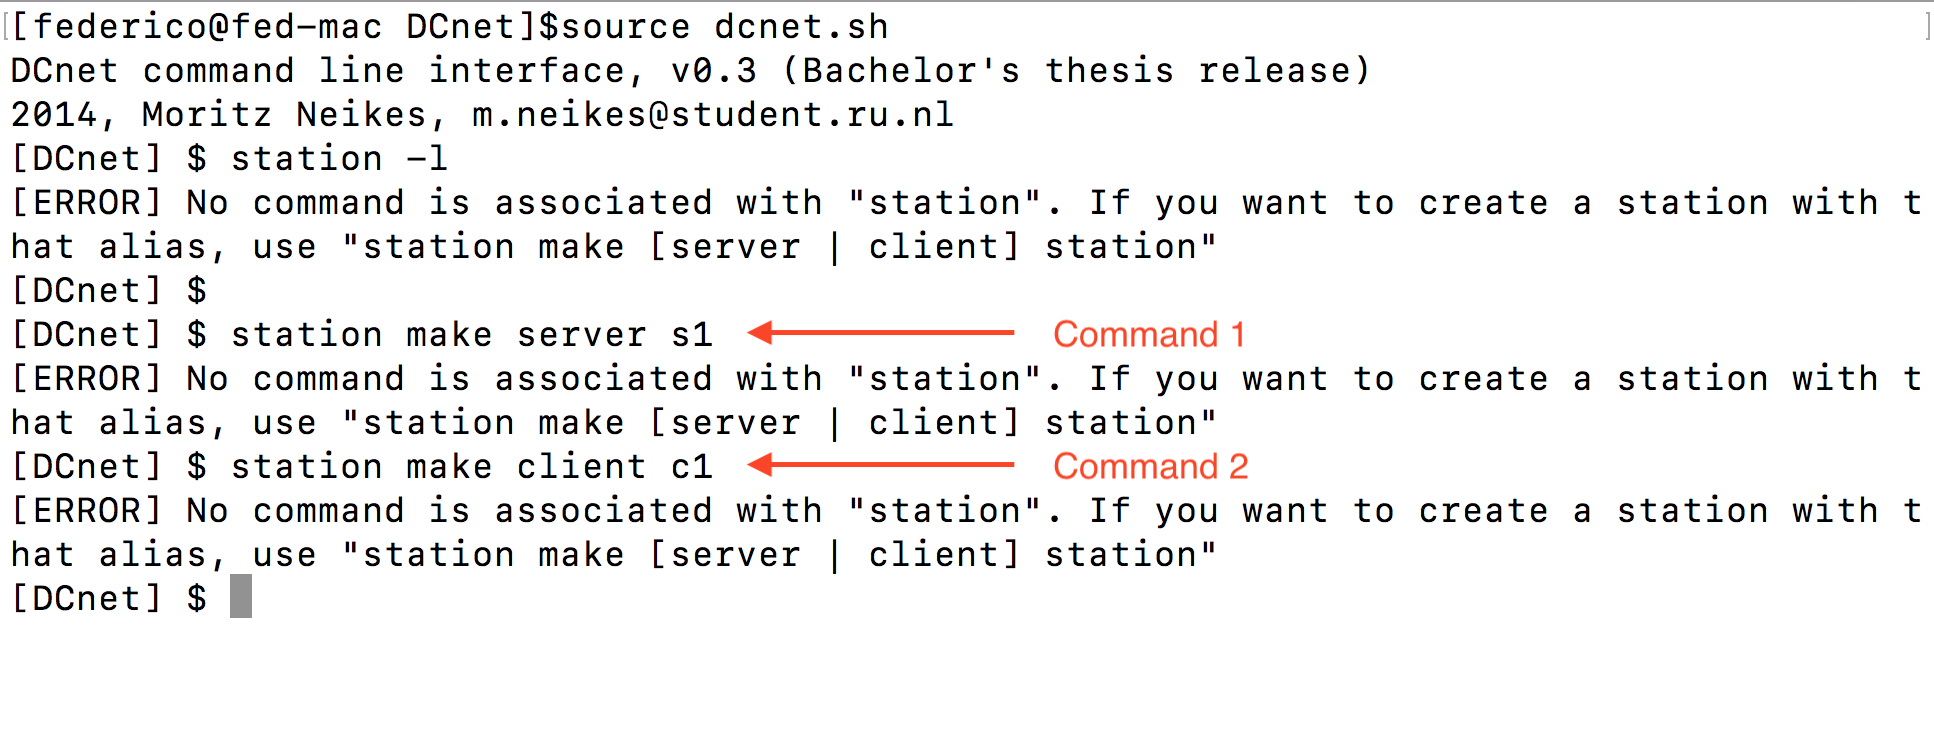
\includegraphics[width=0.7\textwidth]{Images/work1WellDocumentedError.png}
    \caption{Error by following documentation commands.}
    \label{fig:work1error}
\end{figure}

Despite being the best documented project found, there is no setup guide, and the project does not seem to be running in order to solve these issues (last commit over two years ago).

\subsection{Example 2}
Another command line tool found relies on the PubNub as a service to implement the publish subscriber pattern. However, there are no examples of how to configure key files neither on PubNub nor on the documentation of the GitHub project (figure \ref{fig:work2documentation}). Trying to run the software with sample key files results in unhelpful errors(figure \ref{fig:work2error}). 

\begin{figure}[h!]
    \centering
    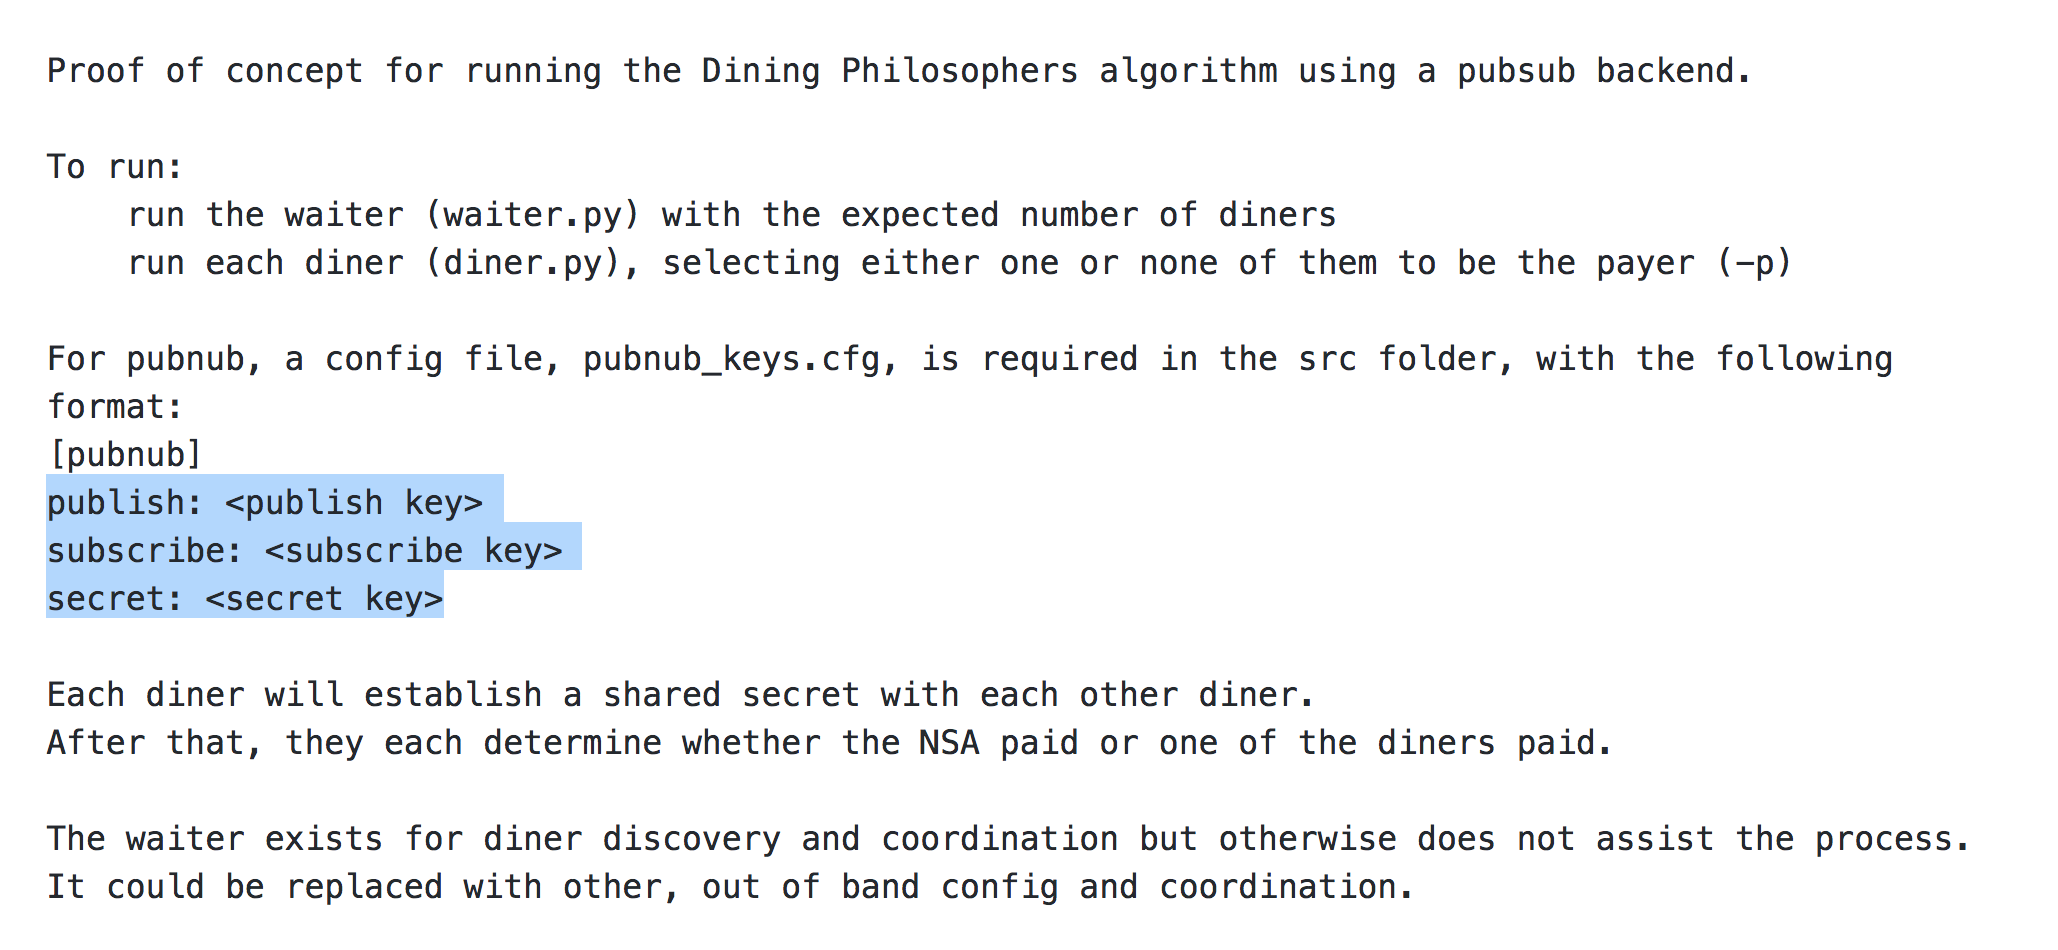
\includegraphics[width=0.7\textwidth]{Images/work2Documentation.png}
    \caption{Documentation instructions but not examples.}
    \label{fig:work2documentation}
\end{figure}

\begin{figure}[h!]
    \centering
    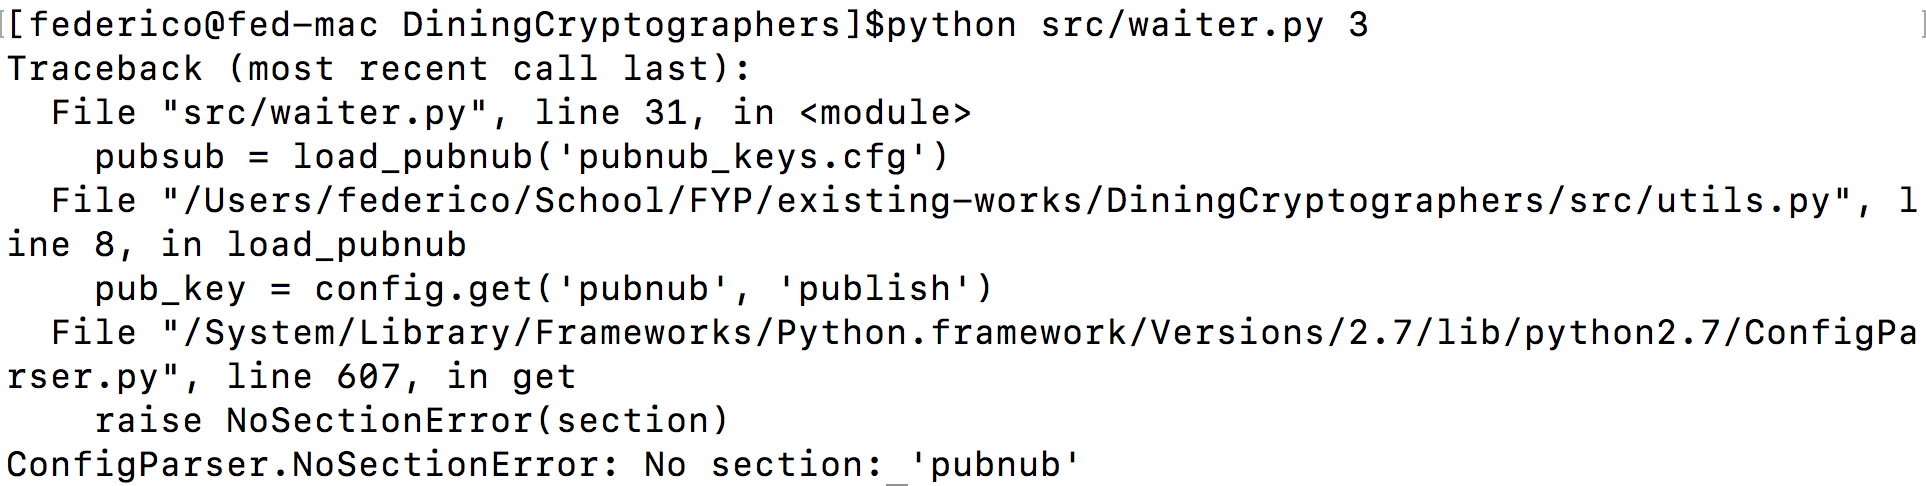
\includegraphics[width=0.7\textwidth]{Images/work2Error.png}
    \caption{Error by trying to run tool with a sample pubnub{\_}keys.cfg.}
    \label{fig:work2error}
\end{figure}

Even if it was to run, this program does not provied a distributed architecture on multiple nodes, so as to resemble closely the multi-party computation.


\subsection{Summary of findings}
The examples shown above were among the best implementations found and they clearly exemplify the lack of practical work on this topic. All projects found are command-line based prototypes. Many of these either present no documentation whatsoever, or do not address fundamental aspects, such as collision detection, in order to encourage a satisfactory discussion for the realistic implementation of a DC-Net. None of them seems to be usable over an actual network, so as to allow multiple users to carry out the protocol.

In the light of these findings, a simulation tool that both illustrates the protocol and investigates the implementations roadblocks is called for.


\chapter{Requirements and Specifications} \label{chapter:requirements}

Following an examination of the working of the Dining Cryptographers protocol, this section focuses on describing the deliverables of the DC-Net simulation. 

Firstly, the requirements to be achieved are presented. They are divided in basic requirements, i.e. the minimum requirements for an acceptable project, and advanced requirements, that instead address the more elaborated technical challenges of the protocol and limitations. In each of these two set of requirements I include a series of functional, non-functional, and security requirements. 

Lastly, the specifications section will explains how each requirement will be implemented.

\section{Brief}
The simulation will be a real-time web-based application that resembles the dynamics of the Dining Cryptographers. The simulation also attempts to be as faithful as possible to the original protocol to preserve untraceability. The website will employ a client-server architecture, with a central DC-Net service . The key-sharing graph topology employed to create a relationship of adjacency among clients is the ring topology.

These design choices will be justified in the design section (chapter \ref{chapter:design}).

\section{Requirements} \label{sec:requirements}
The requirements section, first, informally introduces what the software is going to accomplish, then, it formally lists the results that the simulation is expected to achieve.

\subsection{Basic Requirements}
The basic requirements encompass the necessary features to perform a single round of communication with the only three participants.

\subsubsection{Informal description of the basic protocol at work}
The scenario pictures a server listening to incoming connections. A new client reaches the simulation platform through his computer's browser. When a client connects to the server, the server communicates to all participants the presence of a new user, and when the number of connected nodes is exactly three, the protocol is executed. Further incoming connections are rejected, as the basic protocol acknowledges only three clients. The execution of the protocol entails the following steps:
\begin{enumerate}
    \item The DC-Net Service (the server) generates adjacencies based on the list of connected clients.
    \item The DC-Net Service generates a secret key for each adjacency, and it shares the key with the two clients that belongs to the adjacency over a secure channel;
    \item A client chooses if he wants to flip his response (i.e. send a message); once a client provides his answer, the XOR of his keys and answer are computed and sent back to the server; this process happens for all clients (senders anonymity);
    \item When the server detects that all the responses have been received, the final result is computed by XORing all the responses. This is then broadcasted back to all users (recipient anonymity);
\end{enumerate}

The simulation ends after step four. If throughout the steps mentioned one of the users disconnects, the server halts the protocol execution immediately and this is communicated to the users still in the network. This happens because, as explored in the literature review, anonymity cannot be guaranteed with only two participants.

From this description of how the basic simulation works, I extracted the following lists of basic requirements.

\subsubsection{Functional Requirements}
Functional requirements describe the actual features to be implemented:
\begin{enumerate}
    \item BFUN1 - Allow a user to connect to the DC-Net Service (the server);
    \item BFUN2 - Enable real-time communication among clients and server;
    \item BFUN3 - Inform connected participants when another client joins the network;
    \item BFUN4 - Support exactly the connection of three clients to the DC-Net Service;
    \item BFUN5 - Prompt server to start the protocol execution as soon as three clients are connected;
    \item BFUN6 - Create adjacencies between each pair of neighbouring clients;
    \item BFUN7 - Create a secret key for each adjacency and ensure both clients receive it;
    \item BFUN8 - Allow a client to express their intention of sending a message/flipping their one-bit key;
    \item BFUN9 - Implement the XOR function on the client-side to generate the round response to be sent to server;
    \item BFUN10 - Implement the XOR function on the server-side to generate the final round result;
    \item BFUN11 - Enable server to broadcast the final round result of the protocol execution to all clients;
    \item BFUN12 - If less than three users are connected to the network, inform each participant how many nodes are currently in the network;
\end{enumerate}

\subsubsection{Non-Functional Requirements}
Non-functional requirements are non-technical attributes of the system that are important for the usability of the software: 
\begin{enumerate}
    \item BNFUN1 - Enable the user to understand what is happening at each stage of the protocol with clear messages;
    \item BNFUN2 - Support at least one modern browser;
    \item BNFUN3 - Deploy the system online to allow remote connections like a real distributed application;
    \item BNFUN4 - Distinguish clients between one another with unique names for usability;
    \item BNFUN5 - Slow down the the protocol execution to allow users to understand what is happening in the simulation;
\end{enumerate}

\subsubsection{Security Requirements}
As this is a security protocol it is essential to formalize the necessary security goals to be achieved in this separate section:
\begin{enumerate}
    \item BSEC1 - Implement the key generation process on the centralized DC-Net in a cryptographically secure manner;
    \item BSEC2 - Implement the key exchange over a secure communication channel;
    \item BSEC3 - Abort communication if less than three participants are present;
    \item BSEC4 - Ensure that cryptographers respond to the server with a message that is the XOR of its keys and his message, rather than the message in plain text (so as to enforce sender anonymity);
    \item BSEC5 - Ensure that server employs broadcast/multicast events as often as possible. If unicast messages are used, guarantee that untraceability is not compromised;
\end{enumerate}

\subsection{Advanced Requirements} \label{sec:advancedReq}
The advanced requirements propose possible solutions to some of the limitations of Chaum's basic protocol. Unless addressed, these issues prevent the DC-Net to be applied to a real-world scenario. The final version of the simulation departs from the three-cryptographer one-bit key design. \newline

\subsubsection{Informal description of the advanced protocol at work}
I propose the following advanced features:an arbitrary number of participants in the network, multiple-bit keys and consecutive communication rounds, message collision detection.

\textbf{Arbitrary number of participants:} the protocol can be executed with any number of clients in the network, as long as the minimum number of three clients is present. The protocol execution starts with the generation of adjacencies and the key generation for each of them. Therefore, a client that connects after the beginning of a round has to wait the end of current execution before participating in the communication. In the advent of client disconnection during the protocol, as long as at least three participants are still connected, the system implemented is be resilient enough to complete the round. \newline

\textbf{Longer messages:} the simulation does not terminate after the execution of a single round, but it keeps repeating itself as long as three participants are connected. Moreover, longer keys are used, so that, a client intending to send a message, can XOR his two secret keys with an a number in the same range of the keys as 
DA FARE 
0-255, instead of a 0 or 1 that a 1-bit key permits (see section \ref{sec:longerKeys}). The reason for choosing this key length is to send meaningful human-readable messages by using ASCII encoding. Therefore, a client that in a 1-bit key round would like to flip his message can now send a number in the range 0-255 that will be converted into its corresponding ASCII character. For example, a client wishing to send the character 'a' as his message will XOR his two secret 8-bit keys with the number 97, which is the ASCII-encoded representation of the letter 'a'. Therefore, it is possible transmit actual sentences by repeating rounds with 8-bit keys. \newline

\textbf{Collision detection:} it would not be enough to multiple rounds and longer keys, if the simulator has no capability to detect collisions. 

To expose collisions in a single round, the server stores the keys generated in each round for all clients. 

There is a different

A client that does not intend to send a m


Since a client that does not want to send a message will XOR only his secret keys, the server now can compare the received value with the XOR of the stored key of that client to establish if that user sent a message. The first client to do so will have his message accepted, while all the other clients that will also try to send a message in the same round will be notified that their messages have been rejected. The notification will only be sent after all clients have issued their response. This will avoid a scenario in which the first client to respond to the server sends a message, and the second client to respond also provides a message, but by receiving a rejection notification immediately, the sender would be revealed to a potential eavesdropper of the network. If all clients try to send a message in the same round, even if the notifications of rejection are provided after all clients have issued their response, only the message sender will not receive a rejection notification, and therefore the sender will be again revealed to an eavesdropper. Hence, if all clients try to send a message in the same round, communication is aborted.

To expose collisions across multiple rounds, hence when a client tries to send a sentence one character per round, the proposed method is not enough. To achieve that level of collision detection, the communication will be divided into different types of rounds:
\begin{enumerate}
    \item voting round: single round in which users that would like to send a message will try to win the right to do so. Only one client can win a voting round, who becomes the message sender;
    \item length-calculation round: single round in which the message sender will provide the message he wants to share anonymously. The broadcasted result of this round is only length of the message, which will allow the DC-Net service to generate and share a number of secret keys to each adjacency equivalent to the length of the message. The secret keys of the length-calculation message will be in the range of 100-999. The reason to do so is that if a all generated secret keys would be a number close to 0 the message sender that will try to XOR his keys with a length of message greater than the keys values will be immediately exposed since his response to the server would be the highest value communicated from a client to the server;
    \item communication rounds: as many rounds as the message length happen in which only the message sender is allowed to anonymously XOR a character with his keys. The result of this phase will be an anonymous broadcast of a whole sentence to the whole network.
\end{enumerate}
These three phases will rerun in the same order continuously, and the message sender will not be allowed to win the following voting round, so as to prevent a user to hog the channel of communication.

\subsubsection{Functional Requirements}
\begin{enumerate}
    \item AFUN1 - Support an arbitrary number of participants in the network (instead of just three);
    \item AFUN2 - Repeat rounds of communication continuously;
    \item AFUN3 - Implement longer secret keys;
    \item AFUN4 - Detect multiple senders in the same round to avoid message collisions;
    \item AFUN5 - Divide communication into three types of rounds: voting, length-calculation, communication rounds to be implemented in this order (explained in the design section \ref{sec:designLongMessages});
    \item AFUN6 - Reject clients that did not win the voting round to avoid message collisions in communication rounds;
    \item AFUN7 - Allow user that won the voting round (i.e. message sender) three attempts to provide their own text message in the length calculation round;
    \item AFUN8 - Enable the DC-Net server to create a number of secret keys in bulk, to be shared with the clients before the communication rounds start;
    \item AFUN9 - Convert each letter of the message provided by the message sender client into the corresponding ASCII characters;
    \item AFUN10 - At the termination of communication rounds, display the aggregate message that the user received;
    \item AFUN11 - Prevent the message sender to win the next voting round, so as to ensure a degree of fairness in the network usage;
    \item AFUN12 - Provide help messages to the user to give additional information on the protocol execution;
\end{enumerate}

\subsubsection{Non-functional Requirements}
\begin{enumerate}
    \item ANFUN1 - Increase user-friendliness with some front-end functionalities that empower the user in his learning experience;
    \item ANFUN2 - Allow longer and different types of time intervals between the various stages of communication to ensure that the simulation is understandable;
\end{enumerate}

\subsubsection{Security Requirements}
In addition to the basic security requirements. The following will also be necessary:
\begin{enumerate}
    \item ASEC1 - Keep track of participants secret keys on the DC-Net server in order to detect collisions throughout the upcoming communication rounds;
    \item ASEC2 - Abort communication when the message sender disconnects from the network;
    \item ASEC3 - Abort communication if all participants try to send a message in the same round;
    \item ASEC4 - Synchronize clients' responses for the length-calculation round to avoid the uncovering of the message sender;
    \item ASEC5 - Implement a three-digit key range (100-999) for the length calculation round to ensure hiding of message length (otherwise message sender would be easily spotted if all generated keys were close to 0 and shorter than the message length).
\end{enumerate}


\section{Specifications}
This sections draws upon the listed requirements to delve deeper into \emph{how} they will be implemented.


\subsection{Description of Basic Requirements}

\begin{longtable}[c]{| c | p{4cm} | p{6cm} |}
\caption{Basic Functional Requirements Specifications \label{table:bfun}}

\hline
\multicolumn{3}{| c |}{Begin of Table}\\
\hline
\textbf{Req. Code} & \textbf{Requirement} & \textbf{Specification (how will it be achieved)}\\
\hline
\endfirsthead

\hline
\multicolumn{3}{|c|}{Continuation of Table \ref{table:bfun}}\\
\hline
\textbf{Req. Code} & \textbf{Requirement} & \textbf{Specification (how will it be achieved)}\\
\hline
\endhead

\hline
\endfoot

\hline
\multicolumn{3}{| c |}{End of Table}\\
\hline\hline


\endlastfoot
BFUN1 & Allow a user to connect to the DC-Net Service (the server); & Implement a client-server architecture with node.js and express.js to serve web pages.\\ 
\hline
BFUN2 & Enable real-time communication among clients and server; & Implemented socket.io real-time event-based library to handle communication between clients/server and client.\\
\hline
BFUN3 & Inform connected participants when another client joins the network; & When a connection event happens broadcast to all participants a socket.io 'connection' event, and display the name of the newly connected participant.\\
\hline
BFUN4 & Support exactly the connection of three clients to the DC-Net Service; & Employ control flow so as not to start communication unless there are three active connections; and block further incoming connections.\\
\hline
BFUN5 & Prompt server to start the protocol execution as soon as three clients are connected; & Employ control flow to start communication as soon as three participant are presented, by firing a 'start-round' event from the DC-Net service.\\
\hline
BFUN6 & Create adjacencies between each pair of neighbouring clients; & At the time of a new client addition to the network, renew adjacencies. Employ a list of Adjacency objects to keep track of all neighbouring nodes.\\
\hline
BFUN7 & Create a secret key for each adjacency and ensure both clients receive it; & Implement a random key generator in order to create a common key (either a 0 or a 1).\\
\hline
BFUN8 & Allow a client to express their intention of sending a message/flipping their one-bit key; & Implement a pop-up that explicitly asks the client if they would like to send a message.\\
\hline
BFUN9 & Implement the XOR function on the client-side to generate the round response to be sent to server; & Implement function that XORs the keys of the current round with client's response ('Yes' equates to 1, 'No' equates to 0).\\
\hline
BFUN10 & Implement the XOR function on the server-side to generate the final round result; & Equip server with ability of keeping track of client's result as they are sent to the server. When all clients have expressed their response, automatically computer their XOR.\\
\hline
BFUN11 & Enable server to broadcast the final round result of the protocol execution to all clients; & Immediately after computing the round's result, allow server to broadcast the real message.\\
\hline
BFUN12 & If less than three users are connected to the network, inform each participant how many nodes are currently in the network; & At each connection update the number of nodes needed to start connection, so that a user has a hint of why the communication rounds may have not started.\\
\end{longtable}



\begin{longtable}[c]{| c | p{4cm} | p{6cm} |}
\caption{Basic Non-Functional Requirements Specifications \label{table:bnfun}}

\hline
\multicolumn{3}{| c |}{Begin of Table}\\
\hline
\textbf{Req. Code} & \textbf{Requirement} & \textbf{Specification (how will it be achieved)}\\
\hline
\endfirsthead

\hline
\multicolumn{3}{|c|}{Continuation of Table \ref{table:bnfun}}\\
\hline
\textbf{Req. Code} & \textbf{Requirement} & \textbf{Specification (how will it be achieved)}\\
\hline
\endhead

\hline
\endfoot

\hline
\multicolumn{3}{| c |}{End of Table}\\
\hline\hline

    
\endlastfoot
BNFUN1 & Enable the user to understand what is happening at each stage of the protocol with clear messages; & Instead of executing the protocol just in code, implement user messages on the GUI in order to inform users which stage of the protocol is happening.\\
\hline
BNFUN2 & Support at least one modern browser; & Support Google Chrome as it is the most widely used browser.\\
\hline
BNFUN3 & Deploy the system online to allow remote connections like a real distributed application; & Employ Heorku or AWS hosting services to make the simulation available to the public.\\
\hline
BNFUN4 & Distinguish clients between one another with unique names for usability; & Employ a library for random name generation.\\
\hline
BNFUN5 & Slow down the computer speed in the protocol execution in order to allow the user to understand what is happening in the simulation; & Implement a series of JavaScript timeouts and intervals in order to delay the main steps of the protocol.\\
\end{longtable}


\begin{longtable}[c]{| c | p{4cm} | p{6cm} |}
\caption{Basic Security Requirements Specifications \label{table:bsec}}

\hline
\multicolumn{3}{| c |}{Begin of Table}\\
\hline
\textbf{Req. Code} & \textbf{Requirement} & \textbf{Specification (how will it be achieved)}\\
\hline
\endfirsthead

\hline
\multicolumn{3}{|c|}{Continuation of Table \ref{table:bsec}}\\
\hline
\textbf{Req. Code} & \textbf{Requirement} & \textbf{Specification (how will it be achieved)}\\
\hline
\endhead

\hline
\endfoot

\hline
\multicolumn{3}{| c |}{End of Table}\\
\hline\hline

\endlastfoot
BSEC1 & Implement the key generation process on the centralized DC-Net in a cryptographically secure manner; & Implement a random generator that is cryptographically secure. Main options are node.js basic package \textit{crypto} or the npm library \textit{csprng}\\
\hline
BSEC2 & Implement the key exchange over a secure communication channel; & As this is a web application, securing a communication channel entails making use of \textit{https} protocol to connect to the server and to redirect any \textit{http} (plain text) request to https.\\
\hline
BSEC3 & Abort communication if less than three participants are present; & Implement special broadcast event that resets keys and other information on the clients' browser in order to stop the connection immediately. Use such event when, on a client disconnection event, there are less than three active connections.\\
\hline
BSEC4 & Ensure that cryptographers respond to the server with a message that is the XOR of its keys and his message, rather than the message in plain text (so as to enforce sender anonymity); & Ensure that socket.io events transmit data that is not in 'plain' text.  Hence, transmit messages on which XOR has been applied. \\
\hline
BSEC5 & Ensure that server employs broadcast/multicast events as often as possible. If unicast messages are used, guarantee that untraceability is not compromised; & Employ broadcast events as much as possible, use unicast events only when it does not compromise the untraceability of the message sender.\\
\end{longtable}

\subsection{Description of Advanced Requirement}
\begin{longtable}[c]{| c | p{4cm} | p{6cm} |}
\caption{Advanced Functional Requirements Specifications \label{table:afun}}

\hline
\multicolumn{3}{| c |}{Begin of Table}\\
\hline
\textbf{Req. Code} & \textbf{Requirement} & \textbf{Specification (how will it be achieved)}\\
\hline
\endfirsthead

\hline
\multicolumn{3}{|c|}{Continuation of Table \ref{table:afun}}\\
\hline
\textbf{Req. Code} & \textbf{Requirement} & \textbf{Specification (how will it be achieved)}\\
\hline
\endhead

\hline
\endfoot

\hline
\multicolumn{3}{| c |}{End of Table}\\
\hline\hline

\endlastfoot
AFUN1 & Support an arbitrary number of participants in the network (instead of just three); & Allow more incoming connections to the server and implement control flow in the connection and disconnection handlers to ensure that the correctness of the protocol is preserved when at all times.\\ 
\hline
AFUN2 & Repeat rounds of communication continuously; & After the server completes the protocol execution invoke the function that starts the protocol again. In addition, ensure that all values (e.g. keys) of previous round are cleared both on the clients and the server.\\
\hline
AFUN3 & Implement longer secret keys; & Implement keys in range of 0-1 for voting round, 100-999 for length calculation round; 0-255 for communication rounds. Employ a cryptographically secure method for each of these key generation.\\
\hline
AFUN4 & Detect multiple senders in the same round to avoid message collisions; & Store secret keys on the server and implement control flow to check if any participants has sent a message during a key round.\\
\hline
AFUN5 & Divide communication into three types of rounds: voting, length-calculation, communication rounds to be implemented in this order; & create specialized functions that enable the execution of the different types of round.\\
\hline
AFUN6 & Reject clients that did not win the voting round to avoid message collisions in communication rounds; & Log on the server the list of participants that tried to send a message in the voting round but were not successful. When all response are received, notify them of the rejection.\\
\hline
AFUN7 & Allow user that won the voting round (i.e. message sender) three attempts to provide their own text message in the length calculation round; & Display textbox on message sender's interface to input message, and once provided store it locally on the client's browser.\\
\hline
AFUN8 & Enable the DC-Net server to create a number of secret keys in bulk, to be shared with the clients before the communication rounds start; & employ in-build crypto JavaScript module to create an array of cryptographically secure pseudo random numbers of the desired length. \\
\hline
AFUN9 & Convert each letter of the message provided by the message sender client into the corresponding ASCII characters; & During the computation of a communication round, employ JavaScript built-in string functions to convert a character to its corresponding ASCII value and vice versa.\\
\hline
AFUN10 & At the termination of communication rounds, display the aggregate message that the user received; & Store the result of each communication round locally so that a client can display the whole sentence received.\\
\hline
AFUN11 & Prevent the message sender to win the next voting round, so as to ensure a degree of fairness in the network usage; & record on the client's browser state that a message was previously sent, and display a message accordingly instead of the choice dialog. \\
\hline
AFUN12 & Provide help messages to the user to give additional information on the protocol execution; & Implement question mark icons next to the relevant message parts. Display a detailed message when hovering on the icon.\\
\hline
\end{longtable}



\begin{longtable}[c]{| c | p{4cm} | p{6cm} |}
\caption{Advanced Non-Functional Requirements Specifications \label{table:anfun}}

\hline
\multicolumn{3}{| c |}{Begin of Table}\\
\hline
\textbf{Req. Code} & \textbf{Requirement} & \textbf{Specification (how will it be achieved)}\\
\hline
\endfirsthead

\hline
\multicolumn{3}{|c|}{Continuation of Table \ref{table:anfun}}\\
\hline
\textbf{Req. Code} & \textbf{Requirement} & \textbf{Specification (how will it be achieved)}\\
\hline
\endhead

\hline
\endfoot

\hline
\multicolumn{3}{| c |}{End of Table}\\
\hline\hline
    
\endlastfoot
ANFUN1 & Increase user-friendliness with some front-end functionalities that empower the user in his learning experience; & Alongside the helpful messages feature of AFUN12, enable autoscroll of the simulator interface, and create a small control panel to enable both help message icons and autoscroll.\\
\hline
ANFUN2 & Allow longer and different types of time intervals between the various stages of communication to ensure that the simulation is understandable; & Implement setTimeout and setInterval wrapper functions around the beginning of the main events, such as a new round or protocol restart after abortion.\\
\end{longtable}


\begin{longtable}[c]{| c | p{4cm} | p{6cm} |}
\caption{Advanced  Security Requirements Specifications \label{table:asec}}

\hline
\multicolumn{3}{| c |}{Begin of Table}\\
\hline
\textbf{Req. Code} & \textbf{Requirement} & \textbf{Specification (how will it be achieved)}\\
\hline
\endfirsthead

\hline
\multicolumn{3}{|c|}{Continuation of Table \ref{table:asec}}\\
\hline
\textbf{Req. Code} & \textbf{Requirement} & \textbf{Specification (how will it be achieved)}\\
\hline
\endhead

\hline
\endfoot

\hline
\multicolumn{3}{| c |}{End of Table}\\
\hline\hline

\endlastfoot
ASEC1 & Keep track of participants secret keys on the DC-Net server in order to detect collisions throughout the upcoming communication rounds; & At the time of key generation, store keys in the participant objects; and use compare the XOR of the participant's keys against his round response. \\
\hline
ASEC2 & Abort communication when the message sender disconnects from the network; & include a control flow check in the disconnection handler to identify if the disconnecting client is the message sender and act accordingly.\\
\hline
ASEC3 & Abort communication if all participants try to send a message in the same round; & record if at least one participant did not try to send a message in his round response and employ a control flow check before the publication of the voting round result.\\
\hline
ASEC4 & Synchronize clients' responses for the length-calculation round to avoid the uncovering of the message sender; & trigger a 10 second timer when each client received the length-calculation round keys, so that the interval to dispatch the round response event will be equal for all clients.\\
\hline
ASEC5 & Implement a three-digit key range (100-999) for the length calculation round to ensure hiding of message length; & Provide different minimum and maximum parameters for the csprng.\\
\end{longtable}
\chapter{Design}
This chapter of the report has the purpose of presenting the architecture of the DC-Net simulator from different perspectives through the utilization of UML diagram notations. The overview of the system is still an abstract one, but it is an important step to realize a successful implementation. 

Firstly, the architecture diagrams of the application and examples of the event-based communication will be shown. Following, there is a series of sequence diagrams that exemplifies the data flow between clients and server both for the basic implementation of the protocol and the advanced one.


\section{System Architecture}
The architecture of the simulator is simple.  


\section{Minimal Distributed Architecture}



\section{Event-Based Communication Example}
View from single client point of view.



\section{Basic Data Flow Design}


\section{Advanced Data Flow Design}



\begin{figure}[h!]
    \centering
    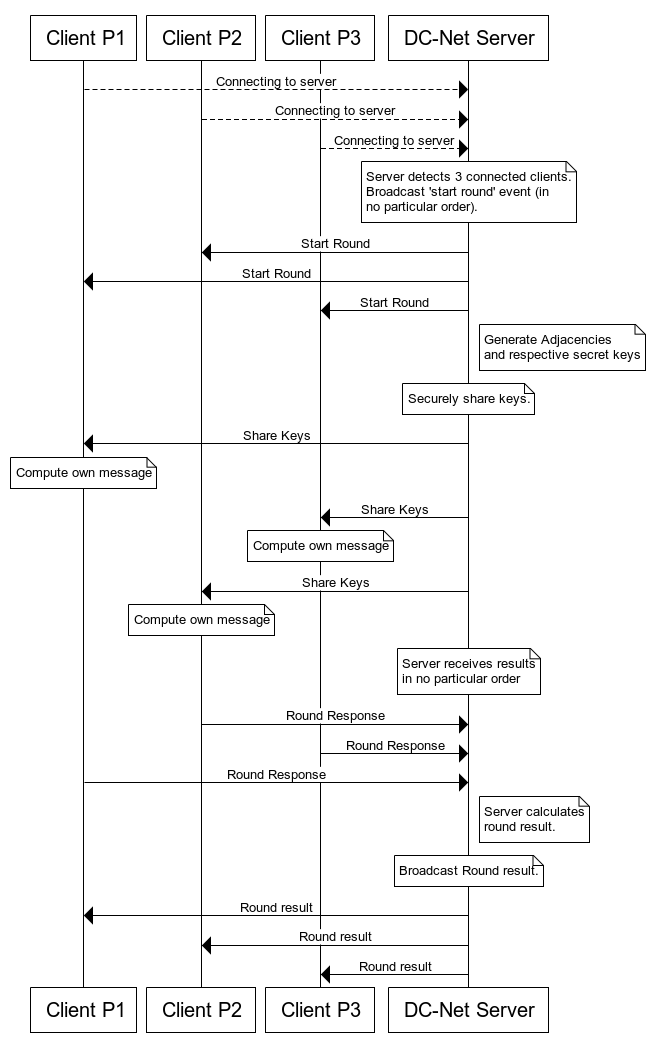
\includegraphics[width=0.8\textwidth]{Images/successfulRound.png}
    \caption{Successful Round of communication.}
    \label{fig:useCaseSuccessfulRound}
\end{figure}

\chapter{Implementation}
This chapter explores the development phase of the simulator following the outlined design structure. The implementation of the project took place in iterations in order to prioritize features and to decrease the overall complexity of implementing all the requirements at once. The complete source code can be found in Appendix \ref{appendix:code}. Appendix \ref{appendix:userguide} explains how to use the simulation tool, and Appending \ref{appendix:setupguide} explains how to run the code locally.


\section{Introducing used Technologies}
This section is an overview of the technologies implemented during the project so as to give a brief introduction of which library or framework has been employed for each part of the architecture.


\subsection{Node.js}
Node.js is JavaScript framework to create servers. It supports useful features such as asynchronous Input/Output, and real-time communication. The ecosystem of this language is the largest collections of open source libraries in the world, called modules. It has been chosen for the simulator because it is specifically designed to create web applications and it has modules for real-time communication and cryptography functions that are the main functionalities needed for the simulation. In addition, it unifies the application with a single main programming language as JavaScript is used both for back-end and front-end development. 


\subsection{Socket.io}
Socket.io is a real-time library for bi-directional communication between clients and servers. The availability of this library only in JavaScript was one of the main reasons to choose Node.js as the preferred server-side environment. This library is based on web sockets, a communication protocol, and it serves as a high-level wrapper to them.

The communication is event-based. Therefore, the some action needs to happen in order to trigger the execution of some code usually stored in an 'event handler' function.
The ease of use of this library makes it easy to create a real-time applications allowing the effort of development to be focused on the security properties that the simulation needs to achieve, rather than being slowed down by how to create a distributed system and exchange messages with low latency.

The library can be used both on the back-end and front-end, so a client and a server can use the same functions (from the API) to trigger or handle events.


\subsection{React.js}
This is another JavaScript library that allows modular development of graphical user interfaces (GUI) in the form of 'components' that can be reused. It is a uncomplicated to create an interface that are interactive and change aspect based on the state of the application.

Therefore, it is a very handy library to create this simulation tool, to create a self-explanatory GUI that will be updated at each stage of the protocol execution.

React.js is used in conjunction with JSX, a special syntax to describe what the UI should look like based on the logic state of the application/component, which is a mixture of HTML and JavaScript.

Since JSX is a special syntax that needs to be 'transpiled' into plain JavaScript and HTML that the browser can understand. In order to do, 'Babel' transpiler will be used through in conjunction with a module bundler technology called 'Webpack'. This latter simply merge together several components created during the development phase into a unique 'bundle' file that will be sent to the browser.

Indeed, the set up for this library is not straightforward, but it is a valuable asset in building a state-based UI.

\subsection{Other third-parties Libraries}
The following are other libraries utilized for significant functionalities of the system that helped both in terms of functionalities and sped up the development phase.

\subsubsection{Cryptographically Secure Pseudo-Random Number Generator (csprng)}
A pivotal code functionality to be implemented successfully is a random generator that produces cryptographically secure numbers to be used as secret keys for each adjacency. A generator that provides this property means that each number is equally likely to be generated, preventing any sort of attack based on the statistical frequency of a stream of generated numbers. 
For this reason, the 'random-number-csprng' library has been implemented, where possible, instead of writing functions that manually generate a random number in a given range.

\subsubsection{Random Name Generator}
The final application will support an arbitrary number of participants connected to the application. In order to identify them among each other a Node library to generate random names has been implemented called 'node-random-name'. 

\subsubsection{Mocha \& Chai}
An important aspect for a mature application is to employ a framework for unit-testing, which is a method to prove the correctness of the logic of an application by verifying the output of a unit being tested is indeed what was expected.

In order to do so in this application, the testing frameworks used is Mocha in conjunction with the assertion library Chai. 


\section{Development Approach}
The approach used throughout the project is a lean methodology that consists in brief iterations of design, implementation and testing. This allowed flexibility to review direction and aims of the initial proposal during project evolution. In addition, making use of iterations helped to be mindful of the time and resource constraints that, as in any other project, were present. Namely, iterations assisted the prioritization of which aspects were more important and what were the dependencies between features to arrange their execution sensibly. This approach lead to the division of the requirements in basic and advanced.


The implementation of functionalities progressed in the following order:
\begin{enumerate}
    \item Implement hard-coded version of the protocol in a single JavaScript file with three participants represented by variables and using a general number random generator;
    \item Develop Node.js web application integrated with React.js and transpiling pipeline of Webpack and Babel;
    \item Integrate Socket.io with React.js for real-time communication;
    \item Distribute the execution of basic protocol between clients and server. Each client possess logic functions inside the main React component (AppComponent). The server generates adjacencies and reacts to events such as connection and disconnection of a client which may trigger the start of the protocol;
    \item Substitute simple random generator with a cryptographically secure pseudo-random number generator;
    \item Implement random name generator to have unique client names;
    \item Introduce objects (Adjacency, Participant, Round) to group functionalities and attributes together and improve modularity of the codebase;
    \item Implement security mechanism to abort communication with less than 3 clients;
    \item Implement clean-up functionalities for the client's browser. This clears keys and other local data when communication is aborted but then restarts again;
    \item Refactor code after having implemented all of the basic features, separating, where possible, the logic of the protocol from the sever-client communication functions;
    \item Implement helper messages on hover for the main steps of the protocol execution;
    \item Start Unit-Testing of the logic functions;
    \item Refactor the AppComponent into smaller React components, each responsible for a single element of the GUI;
    \item deploy application 
    \item Repeat protocol execution continuously, so as to have multiple rounds of communication;
    \item Support connection of an arbitrary number of clients to the server;
    \item Handle connection and disconnection of clients in the middle of round execution;
    \item Implement key storage on the server and utilize this to detect collision;
    \item Implement 8-bit keys;
    \item Divide communication into three types of rounds (voting round, length-calculation round, communication round) and all the relative features that this division entails;
    \item Implement the new security mechanisms needed: prevent the message sender to win the next voting round; abort round when message sender disconnects during round; abort communication if all clients try to send a message in the same round;
    \item Refine user-interface to improve user-friendliness and perform final refactor of codebase;
\end{enumerate}


\subsection{Development Pipeline Tools}
To publish the simulator online, a continuous integration development pipeline was created. This simply means that new features are available live as soon as the codebase updates happen, ensuring that the application is tested correctly. \newline

Firstly, the code is uploaded on Github, a code-sharing platform where a user can store projects.

Secondly, through the presence of a webhook on Github, a code update will trigger the automatic execution of unit-tests in Circle CI (continuous integration). This ensures that new features did not break functionalities previously built.

Lastly, If all tests successful the code is automatically released on the web hosting platform Heroku. The application is in fact available at \url{https://www.dc-net.herokuapp.com}.

\begin{figure}[h!]
    \centering
    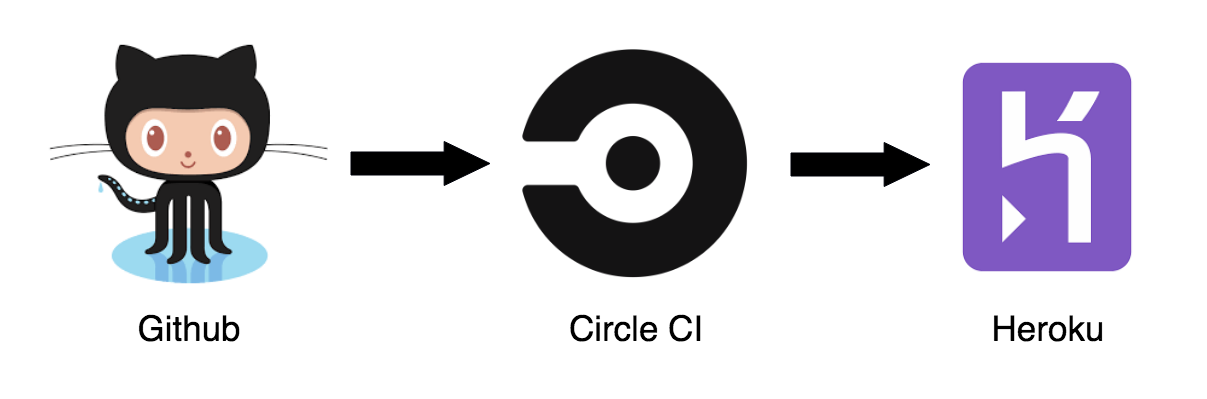
\includegraphics[width=0.70\textwidth]{Images/pipeline.png}
    \caption{Development Pipeline}
    \label{fig:devPipeline}
\end{figure}


\section{Basic Implemented System}
This section presents the simulator components at the competition of the basic requirements.

The website is a single-page application, and when a client connects it tries to join the protocol simulation straight away.




\subsection{Fundamental Security Mechanisms}

\subsubsection{XOR functions}



\begin{lstlisting}
  calculateXORValue(key1, key2, participantMessage) {
    return key1 ^ key2 ^ participantMessage;
  }
\end{lstlisting}


\subsubsection{Abort Communication Control Flow}


\section{Advanced Implemented System}
This sections presents the more complex system achieved at the end of the project with the implementation of all of the advanced requirements.

\subsection{Collision Detection}

\subsection{Handle Connections and Disconnections}

\subsubsection{Browser Connections Limit}

\subsection{Arbitrary number of participants}


\section{Unit Testing}
As previously mentioned, unit testing is the execution of tests on small parts of the codebase, usually one function at a time. This happens by running a given function with some chosen input and comparing the expected output with the actual output. 

Not only unit testing has the main purpose of checking the correct execution of the logic of your application, but it also helps to break down the codebase into separate functions, each one with its specific purpose, since it would otherwise be difficult to test.


NON SO QUESTE DUE SECTIONS
\section{Implementation roadblocks}


\section{Mapping Theoretical Concepts to Implementation}
\chapter{Professional Issues}
This chapter addresses the issues regarding legal, social and ethical issues that arise from the development of this project.

\section{Ethical Concerns}
A fully functioning implementation of the of Dining Cryptographers protocol \textit{can} have a strong impact both legally and socially, due to implications of the existence of a working protocol with unconditional untraceability. However, the software implemented in this project is a simulation of the protocol devised for learning purposes. Despite the software mirrors the internal components of a DC-Net closely, it does not address a number of fundamental issues such as the trust problem that arises from the presence of a server, or the key exchange problem at a protocol level, here solved with https protocol. Therefore there are no ethical implication deriving from this project.


\section{British Computing Society Code of Conduct \& Code of Good Practice}
The project, throughout all of its phases has been observant of the British Computer Society's Code of Conduct. It is important to follow standards and correct practices in order to demonstrate professionalism of one's work. \newline


\textbf{Public Interest:} No group has been discriminated during the execution of the project on the grounds of sex, sexual orientation, marital status, nationality, colour, race, ethnic origin, religion, age or disability. 

In addition, due credit has been given to others' source code whenever required. In particular, it is to be noted that the project file structure was generated by a boilerplate as reported in the appendix. \newline 

\textbf{Professional Competence and Integrity:} The project has been a great opportunity to grow my professional knowledge and skills throughout the whole year, both technically and academically. 

In addition, recurrent alternative points of views were sought to receive valuable criticism to improve the quality of the project. \newline


\textbf{Duty to Relevant Authority:} professional judgment was used to carry out my professional responsibilities with due care and diligence in accordance with King's College London's requirements. 

In addition, none of the part of the project was developed to gain personal benefits. \newline


\textbf{Duty to Profession:} a continuous effort was made to respect the Code of Conduct to uphold the British Computing Society's reputation. \newline 
\chapter{Evaluation}
This chapter contains a personal reflection on the implemented protocol. 

CAMBIA: to present its strength, to assess its contribution to academia,  and weaknesses, to identify possible areas of improvement. 

\section{Assessment on the implementation against the requirements}
The simulation implemented met all the basic requirements and advanced requirements outlined in section \ref{sec:requirements}. Not only the simulation performs the core multi-party XOR computation of three entities, but it also acknowledges several limitations proposing solutions to each one:
\begin{itemize}
    \item message collisions are detected;
    \item the communication occurs in different types of rounds (voting, length calculation and communication) so as to send longer messages;
    \item I adopt ASCII encoding to translate the result of communication rounds into letters so as to communicate human-readable messages;
    \item any number of participants can join or leave the network during the protocol execution without affecting the correctness of the messages exchanged;
\end{itemize}
All of the above takes place with an actual distributed architecture and using a graphical user interface.

I, therefore, consider this a satisfactory implementation.


\section{Comparison of simulation with other works}
Relative to the other implementations found online, my simulation tool implemented proposes some additions that the improve the state of the art of Dining Cryptographer simulated implementations. The main contributions are:
\begin{enumerate}
    \item \textbf{User-experience:} while current tools generally present difficult installation, I provide an easier user experience readily available online. Moreover, the user interface is improved. Current tools mostly offer a command-line interface, which requires the user to \textit{memorise} verbose commands. The user experience provided is, instead, more intuitive with the use of a GUI, which only requires to \textit{recognize} visual cues like buttons and colors. Plus, the simulation is equipped with a number of descriptive messages about what is happening during the execution of the protocol;
    \item \textbf{Documentation}: Tools found provide incomplete or unusable documentation, which may be especially important in understanding a command-line software. The implementation achieved has no remarkable learning barrier but, if needed, a visual user guide is provided (see Appendix \ref{appendix:userGuide});
    \item \textbf{Distributed architecture}: all tools found run locally on a single machine. The simulation implemented offers a realistic experience through the website, since it allows users to connect to the server from different physical locations.
\end{enumerate}

On the whole, this number of improvements move the current state of art forward and enables cryptography enthusiasts learn in a practical way the potential of this protocol.

\section{Known limitations of the implemented solution}
\noindent Despite the improvements, there is a number of known limitations to be acknowledged. 

\subsection{Key Exchange}
As the software has been developed as a web application, \lstinline{https} protocol is the standard way to encrypt traffic over the Internet. \lstinline{Https} provides a solution to exchange keys securely, however, it does not address the problem of key exchange at a protocol level. Such omission is possible because the implementation assumes the channel of communication is the Internet. Therefore, the key-exchange process, at the current state, is not secure within the codebase.

All in all, a more refined solution would settle the key-exchange issue at a protocol level with public key cryptography, such as Diffie-Hellman, or synchronized cryptographically secure pseudo-random number generators (see section \ref{sec:keyExchangeMethods}). This would ensure that, even if this simulation were not web-based, the key-exchange procedure would be secure. However, time constraints played a role in which features I could implement.

\subsection{Collusion}
A real-world scenario that I do not address in this simulation is the possible collusion of malicious participants inside the network. Indeed, attackers could join forces and pool their keys together in order to reveal who the real sender is, as explained in section \ref{sec:disruptionlimitation}. A system that also addresses this issue needs complex mechanisms such as a tree-like overlay network \cite{Wang}, that are beyond the scope of this project.

\subsection{Presence of Server} \label{sec:evalServerPresence}
Making use of a client-server architecture introduces the entity of the server, which represents the DC-Net Service. This raises the issue of trust and it calls for an assumption that, at server level, there is no abuse of the comprehensive view of the network (see section \ref{sec:clientserver}). Since this is a web application, the use of a SSL certificate would verify the server's identify but a client using this platform cannot know how the server handles the responses sent to it. I made a design choice between the useful but questionable presence of an omniscient principal, the server, and the choice of a serverless architecture but with limited capabilities. The client-server architecture was chosen because the presence of a centralised service allows the implementation of some advanced features. For example, it would not be possible to detect collisions without an entity that is able to see all the messages in a round.

\subsection{Collision Detection Warnings: Effects} \label{sec:collisionDetectionWarnings}
In my implementation, I divided communication in three types of round (voting, length-calculation, communication rounds) as presented in section \ref{sec:advancedReq}.
As presented in XX, a collision detection warning is sent solely to the failing participants who attempted to win a voting round. Although I justify the necessity of such mechanism (section XX), I came to realise that there are implications in respect to untraceability, which cannot be overlooked.


\subsubsection{Anonymity Reduction} \label{sec:anonymityReductionLimitation}
Anonymity, as we have seen, is not an absolute concept; rather, it depends on the number of participants inside the anonymity set (section \ref{sec:anonymityset}), 

During a critical review of the features implemented, I found out that 'rejection warning' notifications reduce the sender anonymity set because an eavesdropper can deduct that none of the clients who received such notification is the potential real sender. It follows that the anonymity set is reduced to those participants not receiving such warning notification. As a result, sender anonymity is reduced.

The reality is that there is no easy workaround to maintain the degree of anonymity unaffected. Hypothetically, if the user experience would be sidelined, the server could simply drop the unsuccessful attempts to win the voting round and not send a rejection warning message back. However, there must still be an update of state of the client's browser to change their sender status so that there is no prompt to send a message, and this can come only from the server.

\subsubsection{Edge case of anonymity impairment} \label{sec:anonymityImpairmentEdgeCase}
I also found an edge case, where an eavesdropper inside the network can impair the internal untraceability of a round due to the same 'rejection warning' notifications. The edge case scenario consists of three cryptographers with the following features: 

\begin{enumerate}
    \item a message sender who won the voting round;
    \item a second participant that tried to win the voting round;
    \item a third participant, eavesdropping, who can listen in to all communication from and to the server.
\end{enumerate}
It follows that, since there are only two participants other than the eavesdropper, then the eavesdropper knows that the message sender obviously is the client who did not receive a rejection. In this case, anonymity is internally breached and only 'preserved' in respect to an external observer, assuming that such observer is not colluding with the internal eavesdropper.


\section{Discrepancy between Protocol Perfection and Real World Implementation}
The principle objective of this project has been to demonstrate the existence of a disparity between the theoretical perfection of the DC-Net security protocol and the fallibility of a working solution that tries to hold the desired security properties and preserve correctness at all times. I aimed to show this divergence by creating a simulation tool for the protocol in question. The effort of putting a theoretical protocol in practise, i.e. overcoming complications that arose during each step of development, has triggered a series of reflections. Put together, these observations on the work performed, represent a complementary contribution to the wealth of academic papers on the DC-Net protocol, which focus almost entirely on theoretical considerations. 

The rest of the chapter gives space to fundamental practical challenges, too often neglected in the theoretical literature.

\subsection{Correctness of protocol execution}
The protocol in theory is presented by Chaum with cryptographers at the table. In an actual implementation, there is the process of sitting down at the table. In other words, there is a connection event for each client to the DC-Net Service, and therefore a temporal element in joining the network, which may take place at different phases of the protocol execution. Such element can, in practise, create an issue of correctness when one or more participants join or leave the protocol during the actual execution.

\subsubsection{Correctness of protocol on client connection during protocol execution}
Adding a participant to the graph implies updating the adjacencies of the graph, i.e. renewing the secret keys between clients. If a connection of a $nth$ client happens when the protocol started and some, but not all, participants already provided their responses, then, performing an update of adjacencies at this stage would create a mismatch of state between the clients and the server.

More specifically, after the keys updated, the combination of old responses recorder by the server in conjunction with the missing responses of that will now be provided to the server will not XOR each other out, therefore affecting the correctness of the protocol.

Thus, the simulations employs a waiting mechanism for clients that join the network in the midst of the protocol execution to delay their participation until the next voting round.

\subsubsection{Correctness of protocol on client disconnections}
Another important problem not addressed by theoretical works is the event of disconnection of a user while the protocol is executing. A client abandoning the network after the key-exchange phase in either of the voting, length-calculation, or communication rounds undermines the correctness of the final result because the response of the disconnecting client is excluded in the server's final round calculation. This leads to an incorrect round results since some of the secret keys are not XORed twice, which is fundamental to reveal the broadcasted hidden round message (an ASCII character) sent by the anonymous message sender (see section \ref{sec:xorDemonstration}).

The immediate solution is to, again, update the adjacencies when a client disconnects and, if necessary, stop and restart the round. However, in a network with $n$ number of participants, such mechanism would affect the user experience and serviceability of the protocol. Moreover, it also allows a malicious participant to harm the availability of the service by simply connecting and disconnecting to the service repeatedly.

It is in these circumstances that the presence of the DC-Net service is valuable. That is, when a disconnection occurs, the server that keeps track of all of the adjacencies' keys, simply updates the two relevant adjacency objects and their respective keys, without interrupting the round in progress.

\subsection{Edge cases that compromise untraceability}
The protocol in principle describes the minimum set of communication steps necessary for a smooth round of communication. However, in a real world scenario, it is very likely that more messages or events are exchanged between a client and the server. For instance, a relevant case is the 'collision detection warning' notification, (section \ref{sec:collisionDetectionWarnings}), which affects the degree of untraceability, by reducing the sender anonymity set. 

Although I presented this example in the known limitations of my simulator, this complication is very likely to be encountered in any attempt of implementing this protocol. The more complex an implementation is, the higher the likelihood of compromising untraceability by introducing new communication steps. Therefore, guaranteeing untraceability for all edge cases in practical implementations is more laborious than ensuring the perfection of the cryptographic algorithm at a theoretical level. 


\subsection{Necessity of a length-calculation round}
A proposal to extend the protocol to multiple rounds of communications is offered by many academic figures. This divides communication in a voting phase and a actual sending phase.

Although this approach is the same proposed for my implementation, I identified the necessity of a third type of round was identified: length-calculation round. This leads to a division of the protocol execution in voting, length-calculation and communication rounds. The newly introduced round type has the purpose of allowing the message sender to communicate the length of the sentence to the server without being traced by potential eavesdroppers. I deemed this step necessary, since in my implementation the server needs to compute the same number of keys as the length of the sentence before the communication rounds start. Without this intermediate round type, a message sender that will directly communicate the length of the message to the server would be trivially identified by an eavesdropper.

The need of this step was never found in the theoretical works that simply propose to divide the protocol in voting and communication rounds.


\subsection{Difficulty of ensuring fair use of network}
DC-Net protocol focuses on untraceability. When looking at the implementation of a software, however, another main security goal to be guaranteed is availability. In the context of the implemented simulation, a malicious participant could decide to hog the service and make it unavailable by continuously attempting to win the voting round. To counteract this issue, I implement a feature that prevents the message sender to win the next voting round. By doing so, a malicious participant trying to hog the service, can succeed only half of the time (one round yes and one round no).

However, the ideal solution to ensure fairness in the network usage is to implement a queue. The server would make use of this data structure to record the chronological order of attempts by the participants to send a message. This gives the possibility to a participant to send a message when he reaches the front of the queue. Though, this is a very fiddly feature to implement due to intricate possible scenarios. 


An exemplification of this is the following: there are at least two cryptographers in the sending queue who tried to win the voting round simultaneously. At the start of the new round the user at the front of the queue is asked if he would still like to send a message. The first issue raised is that this question cannot be a unicast message between the client and the server. Otherwise if after this communication the length-calculation round happens, it would be obvious who the sender is. Therefore, to maintain untraceability this question would require a further type of broadcast round. 

Furthermore, there are particular edge cases to be addressed. For example, what happens if the cryptographer, front of the queue, accepted to send a message but then disconnects? It is likely that that the same offer of sending a message should be made to the new first user in the queue, having to repeat another broadcast round just to ask this. Hence, implementing a queue of message senders risks to make the protocol to repeat the voting phase several times. This is the completely counterproductive since it could affect the availability of the service ,which was the issue that the queue set out to solve in the first place. 

This is an excellent instance of how an implementation can get highly difficult rather quickly. \newline \newline




Ultimately, all these various exemplifications of differences between a theoretical protocol and an effective application illustrated the constructive knowledge gained along the hands-on development phase. The purely theoretical argumentation of the protocol presented in many papers rarely offer an appreciation of these practical complex challenges. Hence, these were important remarks to be addressed as a contribution to the academic community.


\chapter{Conclusions and Future Works}

\section{Conclusions}

The main goal of this report has been to display the challenges of implementing Chaum's protocol in practice, as this has never been seriously attempted before. Specifically, I have tried to show how a working implementation inevitably puts strain on the security properties of untraceability as well as correctness. 

Embarking on a simulation project for the DC-Net protocol was a necessary step to expose the difficulties of maintaining untre ...

As I have addressed in chapter 2, theoretical accounts do not seem to be aware of some of the issues I pointed out, namely preserving correctness when clients join/leave network during protocol execution, the need of a length-calculation round between voting phase and communication phase; how to transmit useful messages. 
 
 The literature I reviewed, however, positive in supplementing Chaum's protocol with interesting solution for the key exchange phase; solution for identifying malicious attackers;
 
Nonetheless, since the academic debate stays in the abstract and do not dare to sail the dangers waters of the real-world, there is only so far that you can go. 


The very few attempts to build a simulation are not committed. Most tools seem uncompleted attempts to simulate the protocol, 


My work sits in this space very originally. 

I aimed at building a very usable tool, and in the early stages I had to take a number of design choices. Thinking about the protocol in realistic term to have a working implementation I met some roadblocks for which I came up with my own design choices. 

I then proceeded to implement such design in the form of a web application, that clearly addressed all the weakneesses of similar solution. 

Because there is a certain complexity to translate the concepts from theory to practise, the project was divided in basic and advanced requirement as a form of prioritization. 


The implementation met all the intended requirements both the basic ones, for an acceptable product, and the advanced ones, for a more complex system with useful functionalities. A number of roadblocks arose throughout the development of the project: - metti i roadblocks. 

 The effort of putting a theoretical protocol in practice, i.e. overcoming complications that arose during each step of development, has triggered a series of reflections. Put together, these observations on the work performed, represent a complementary contribution to the wealth of academic papers on the DC-Net protocol, which focus almost entirely on theoretical considerations.

The overarching theme throughout the paper has been that there is a disparity between the theoretical perfection of the DC-Net protocol and the practical difficulties of deployment. 
 I have not resolved this gap but I clearly show that it is not possible to overcome the complications of the real world with the same perfection of the theory. 
 
 deemed unpractical but my attempt to make it 2work shows a lot of untackled areas that are important to address and I hope this triggers a discussion closer to the real world. 
 
 
 I have contextualised the issue of anonymity vs untraceability, due to the fact that these are difficult concepts to reason about. 
 
 (Anonymity entail untraceability but not vice versa. Therefore anonymity is a stronger form of untraceability.
 
 
 The report started with a conceptual distinction between anonymity and untraceability.
 
 
 




The report started giving an in-depth presentation of this security protocol, to then move to the explanation of the implementation process, starting from design and ending with testing. 

The need to develop such a tool was found in the lack of interesting practical works on this protocol, which is however addressed extensively by academic theoretical works. 


As a consequence of meeting these challenges, my contributions are: a proposal of diving the communication in voting, length-calculation and communication round (instead of voting and communication rounds); detecting collision by storing secret keys on the server; using 8-bit keys that allow a message to be any number from 0 to 255, which allows to interpret an anonymously shared message with the EASCII encoding standard in order to share useful human-readable messages. In addition, also the simulation tool published live at \url{https://www.dc-net.herokuapp.com} is a practical contribution for the community. 

Most importantly, the difficulties encountered during the development expanded further the goal of creating a simulation tool by also offering, as a contribution, an analysis presented in the evaluation which appreciates the discrepancy between theory and implementation of the Dining Cryptographers protocol.



\section{Future Works}
There are a number of future works to recommend in order to further move the simulation closer to a fully working implementation of the protocol.


\subsection{Server Trust Issue}
how? ssl for authentication

\subsection{Secure Key-Exchange at protocol level}
Diffie-Hellman

\subsection{Detect Collusion}
Fail-Stop key Generation

\subsection{Session object wrapper}





%%%%%%%%%%%%%%%%%%%%%%%%%%%%%%%%%
% References
%%%%%%%%%%%%%%%%%%%%%%%%%%%%%%%%%
\bibliographystyle{plain}
\bibliography{references}
\addcontentsline{toc}{section}{Bibliography}
\begin{thebibliography}{99}

\bibitem{Chaum} Chaum, D. (1988). The dining cryptographers problem: Unconditional sender and recipient untraceability. Journal of Cryptology, [online] 1(1). Available at: http://www.cs.ucsb.edu/~ravenben/classes/595n-s07/papers/dcnet-jcrypt88.pdf [Accessed 10 Mar. 2017].

\bibitem{Anonymity} Oxford Dictionary of English, "Anonymity", 2017

\bibitem{Malkhi} D. Malkhi, "Advanced Course in Computer and Network Security", Jerusalem 2002 - http://www.cs.huji.ac.il/~ns/Anonymity.pdf

\bibitem{Pfitzmann} A. Pfitzmann, M. Kohntop,"Anonymity, Unobservability, and Pseudonymity – A Proposal for Terminology", Germany 2001

\bibitem{Franck} C. Franck, "New Directions for Dining Cryptographers", Luxembourg 2008 - https://secan-lab.uni.lu/images/stories/christian{\_}franck/FRANCK{\_}Christian{\_}Master{\_}Thesis.pdf

\bibitem{Diffie1} W. Diffie, M. E. Hellman, "New Directions in Cryptography", 1976 https://ee.stanford.edu/~hellman/publications/24.pdf

\bibitem{Fischer} Fischer-Hubner, S. (2001). IT-security and privacy. Berlin: Springer, pp.125-128.

\bibitem{Lewin} M. Lewin, "ACCU - All About XOR", 2012 https://accu.org/index.php/journals/1915

\bibitem{Scholz} I. Scholz, "Dining Cryptographers - The Protocol", http://www.eigenheimstrasse.de/svn/dc

\bibitem{wiki1} Wikipedia, "Secure multi-party computation". https://en.wikipedia.org/wiki/Secure{\_}multi-party{\_}computation

\bibitem{Golle} P. Golle, A. Juel, "Dining Cryptographers Revisited", 2004, https://www.freehaven.net/anonbib/cache/golle:eurocrypt2004.pdf 

\bibitem{Waidner} M. Waidner, "Unconditional sernder and recipient untraceability in spite of active attackers", Universitat Karlsruhe, 1989, https://link.springer.com/content/pdf/10.1007/3-540-46885-4{\_}32.pdf

\bibitem{XORJS} Microsoft Docs, "Bitwise XOR Operator ($\wedge$)", \url{https://docs.microsoft.com/en-us/scripting/javascript/reference/bitwise-xor-operator-decrement-hat-javascript}

\bibitem{Susilo} Safavi-Naini R.
 Susilo W. ,"General Construction for Fail Stop A Signatures using Authentication Codes"

\bibitem{Souders} Steve Souders, "Roundup on Parallel Connections", \url{http://www.stevesouders.com/blog/2008/03/20/roundup-on-parallel-connections/}

\bibitem{Nodejs} Node.js Foundation, "About Node.js", \url{https://nodejs.org/en/about/}


\end{thebibliography}



%%%%%%%%%%%%%%%%%%%%%%%%%%%%%%%%%
% Appendices
%%%%%%%%%%%%%%%%%%%%%%%%%%%%%%%%%
%\appendix
%\chapter{User Guide}
\section{Instructions}
To run the system please follow the steps below:
\begin{enumerate}
\item Start backend/nodeserver/server.js
\item Start backend/MLServer/MLServer.jar
\item Start IPS\_Admin app and create buildings+rooms.
\item Measure rooms using the IPS\_Admin. After the measurements are done, press the learn button in BuildingActivity
\item The MuseumGuide app can now be used to locate the device.
\end{enumerate}
%\chapter{Example Files}

\section{domain.pddl}
\begin{lstlisting}
(define (domain museum)
(:requirements :typing :durative-actions :fluents)
(:types
    exhibit person - object
)
(:predicates
    (at ?p - person ?e - exhibit)
    (path ?e1 ?e2 - exhibit)
    (want-to-see ?e - exhibit)
    (visited ?e - exhibit)
    (open)
)
(:functions
    (time-to-walk ?e1 ?e2 - exhibit)
    (time-to-see ?e - exhibit)
    (excitement ?e - exhibit)
    (seen)
)

(:durative-action walk
  :parameters
   (?p - person
    ?e1 ?e2 - exhibit)
  :duration (= ?duration (time-to-walk ?e1 ?e2))
  :condition
   (and (over all (path ?e1 ?e2)) (at start (at ?p ?e1)) (over all (open)))
  :effect
   (and (at start (not (at ?p ?e1))) (at end (at ?p ?e2))))

(:durative-action view
  :parameters
   (?p - person
    ?e - exhibit)
  :duration (= ?duration (time-to-see ?e))
  :condition
   (and (over all (at ?p ?e)) (at start (want-to-see ?e)) (over all (open)))
  :effect
   (and (at start (not (want-to-see ?e))) (at start (increase (seen) (excitement ?e))))
)


)

\end{lstlisting}
\newpage

\section{problem.pddl}
\begin{lstlisting}
(define (problem simplemuseum)
(:domain museum)
(:objects
    visitor - person
    e0 e1 e2 - exhibit
)
(:init
(want-to-see e0)
(want-to-see e1)
(want-to-see e2)
(path e0 e1) (path e1 e0)
(= (time-to-walk e0 e1) 0)
(= (time-to-walk e1 e0) 0)
(path e0 e2) (path e2 e0)
(= (time-to-walk e0 e2) 0)
(= (time-to-walk e2 e0) 0)
(path e1 e2) (path e2 e1)
(= (time-to-walk e1 e2) 0)
(= (time-to-walk e2 e1) 0)
(= (time-to-see e0) 16)
(= (time-to-see e1) 12)
(= (time-to-see e2) 0)
(at visitor e0)
(= (seen) 0)
(= (excitement e0) 1)
(= (excitement e1) 1)
(= (excitement e2) 1)
(open)
(at 10000 (not (open)))
)
(:goal (and
;(visited e0)
;(visited e1)
;(visited e2)
)
)
(:metric maximize (seen))
)
\end{lstlisting}
\newpage

\section{learning.arff}
\begin{lstlisting}
@relation room

@attribute 54:22:f8:17:9a:db NUMERIC
@attribute 00:91:f9:4b:44:e0 NUMERIC
@attribute e2:91:f9:4b:44:e0 NUMERIC
@attribute c0:3e:0f:85:ab:9d NUMERIC
@attribute 00:91:f9:4b:44:e1 NUMERIC
@attribute 22:91:f9:4b:44:e1 NUMERIC
@attribute 2c:39:96:b4:c3:a6 NUMERIC
@attribute 44:e9:dd:6d:36:83 NUMERIC
@attribute 5c:7d:5e:0e:4b:cf NUMERIC
@attribute c2:91:f9:4b:44:e0 NUMERIC
@attribute class {5713ab468794d11d17c53d59,5713aa0e8794d11d17c53d57,5713aa6b8794d11d17c53d58,5713abae8794d11d17c53d5a}
@data
-47.0,-66.0,-60.0,-54.0,-76.0,-76.0,-86.0,-80.0,-67.0,-64.0,5713ab468794d11d17c53d59
-47.0,-66.0,-60.0,-48.0,-78.0,-78.0,-80.0,-84.0,-67.0,-64.0,5713ab468794d11d17c53d59
-45.0,-64.0,-63.0,-56.0,-88.0,-87.0,-88.0,-81.0,-79.0,-64.0,5713aa0e8794d11d17c53d57
-42.0,-71.0,-66.0,-52.0,-86.0,-86.0,-84.0,-83.0,-63.0,-69.0,5713aa0e8794d11d17c53d57
-47.0,-77.0,-74.0,-61.0,-90.0,0.0,-77.0,-79.0,-69.0,-73.0,5713aa6b8794d11d17c53d58
-54.0,-76.0,-74.0,-60.0,-90.0,0.0,-77.0,-74.0,-72.0,-73.0,5713aa6b8794d11d17c53d58
-28.0,-72.0,-67.0,-60.0,-90.0,-90.0,-73.0,0.0,-47.0,-73.0,5713abae8794d11d17c53d5a
-35.0,-70.0,-70.0,-59.0,-91.0,-90.0,-71.0,-87.0,-54.0,-73.0,5713abae8794d11d17c53d5a

\end{lstlisting}
\newpage

\section{unclassified.arff}
\begin{lstlisting}
@relation room

@attribute 54:22:f8:17:9a:db NUMERIC
@attribute 00:91:f9:4b:44:e0 NUMERIC
@attribute e2:91:f9:4b:44:e0 NUMERIC
@attribute c0:3e:0f:85:ab:9d NUMERIC
@attribute 00:91:f9:4b:44:e1 NUMERIC
@attribute 22:91:f9:4b:44:e1 NUMERIC
@attribute 2c:39:96:b4:c3:a6 NUMERIC
@attribute 44:e9:dd:6d:36:83 NUMERIC
@attribute 5c:7d:5e:0e:4b:cf NUMERIC
@attribute c2:91:f9:4b:44:e0 NUMERIC
@attribute class {5713ab468794d11d17c53d59,5713aa0e8794d11d17c53d57,5713aa6b8794d11d17c53d58,5713abae8794d11d17c53d5a}
@data
-41.0,-71.0,-67.0,-52.0,-86.0,-86.0,-86.0,-82.0,-63.0,-69.0,?


\end{lstlisting}
\newpage

\section{RPs.data}
\begin{lstlisting}
54:22:f8:17:9a:db
00:91:f9:4b:44:e0
e2:91:f9:4b:44:e0
c0:3e:0f:85:ab:9d
00:91:f9:4b:44:e1
22:91:f9:4b:44:e1
2c:39:96:b4:c3:a6
44:e9:dd:6d:36:83
5c:7d:5e:0e:4b:cf
c2:91:f9:4b:44:e0
\end{lstlisting}
\newpage

\section{rooms.data}
\begin{lstlisting}
5713ab468794d11d17c53d59
5713aa0e8794d11d17c53d57
5713aa6b8794d11d17c53d58
5713abae8794d11d17c53d5a
\end{lstlisting}
\newpage

\end{document}
